\documentclass{article}
\usepackage[preprint]{neurips_2024}

% -----------------------
% Page + typography (arXiv-ish)
% -----------------------
\usepackage[T1]{fontenc}
\usepackage{lmodern}
\usepackage{microtype}

% -----------------------
% Math
% -----------------------
\usepackage{amsmath, amssymb}

% -----------------------
% Figures / floats
% -----------------------
\usepackage{graphicx}
\usepackage{float}

% -----------------------
% Lists / comments
% -----------------------
\usepackage{enumitem}
\usepackage{comment}

% -----------------------
% Links (clean, no ugly boxes)
% -----------------------
\usepackage[hidelinks]{hyperref}

% -----------------------
% TikZ
% -----------------------
\usepackage{tikz}
\usetikzlibrary{matrix, calc, positioning, arrows.meta}

% -----------------------
% Code listings
% -----------------------
\usepackage{listings}
\usepackage{xcolor}

\definecolor{codegray}{rgb}{0.5,0.5,0.5}
\definecolor{codegreen}{rgb}{0,0.6,0}
\definecolor{codepurple}{rgb}{0.58,0,0.82}
\definecolor{backcolour}{rgb}{0.95,0.95,0.92}

% Google Colab-like colors
\definecolor{colabKeyword}{rgb}{1,0.6,0.6}
\definecolor{colabString}{rgb}{0.19,0.55,0.91}
\definecolor{colabComment}{rgb}{0.5,0.5,0.5}
\definecolor{colabBackground}{rgb}{0.17,0.17,0.17}
\definecolor{colabText}{rgb}{0.77,0.77,0.77}

\lstdefinestyle{colabstyle}{
    backgroundcolor=\color{colabBackground},
    commentstyle=\color{colabComment}\ttfamily,
    keywordstyle=\color{colabKeyword}\ttfamily,
    stringstyle=\color{colabString}\ttfamily,
    basicstyle=\color{colabText}\ttfamily\footnotesize,
    numbers=left,
    numberstyle=\tiny\color{colabText},
    numbersep=5pt,
    breaklines=true,
    breakatwhitespace=false,
    keepspaces=true,
    showspaces=false,
    showstringspaces=false,
    showtabs=false,
    tabsize=2,
    captionpos=b,
    language=Python
}
\lstset{style=colabstyle}

% -----------------------
% Title block
% -----------------------
\title{A Synthesizable RTL Implementation of Predictive Coding Networks}
\author{
Timothy Oh \\
University of California, Riverside
}
\date{August 2025}

\raggedbottom

\begin{document}
\maketitle

\begin{abstract}
Backpropagation has enabled modern deep learning but is difficult to realize as an online, fully distributed hardware learning system due to global error propagation, phase separation, and heavy reliance on centralized memory. Predictive coding offers an alternative in which inference and learning arise from local prediction-error dynamics between adjacent layers. This paper presents a digital architecture that implements a discrete-time predictive coding update directly in hardware. Each neural core maintains its own activity, prediction error, and synaptic weights, and communicates only with adjacent layers through hardwired connections. Supervised learning and inference are supported via a uniform per-neuron clamping primitive that enforces boundary conditions while leaving the internal update schedule unchanged. The design is a deterministic, synthesizable RTL substrate built around a sequential MAC datapath and a fixed finite-state schedule. Rather than executing a task-specific instruction sequence inside the learning substrate, the system evolves under fixed local update rules, with task structure imposed through connectivity, parameters, and boundary conditions. The contribution of this work is not a new learning rule, but a complete synthesizable digital substrate that executes predictive-coding learning dynamics directly in hardware.
\end{abstract}

\paragraph{Artifact availability.}
A complete reference implementation of the architecture described in this paper
is available as open-source RTL together with simulation testbenches and
reproducibility scripts at

\begin{center}
\url{https://github.com/alskaf1293/neuralcomputer}
\end{center}

The repository contains synthesizable SystemVerilog implementations of the
neural core, layer composition modules, and multi-layer network construction,
along with Verilator-based testbenches that reproduce the experiments reported
in Section~\ref{sec:experiments}. Each experiment produces CSV learning curves
that can be plotted directly to regenerate the figures in this paper.

\section{Introduction}
\label{sec:intro}

Modern machine learning systems are typically trained by backpropagation, which computes gradients by combining global loss information with a tightly coordinated forward/backward computation schedule. Although highly effective, this paradigm is difficult to realize as a fully distributed learning substrate in hardware. The backward pass requires structured global error propagation, intermediate activation storage, and substantial movement of data through memory and interconnect.

Predictive coding offers an alternative formulation in which inference and learning arise from minimizing prediction errors across a hierarchy \cite{rao1999predictive, friston2005theory}. In standard predictive coding networks (PCNs), each layer predicts the layer below; each unit updates its state and synaptic weights using only locally available quantities: its own activity, its own prediction error, presynaptic activity from the adjacent layer above, and prediction errors from the adjacent layer below. This locality makes predictive coding attractive as a candidate algorithmic substrate for physically embedded learning systems.

This paper presents a digital micro-architecture that directly implements predictive coding equations at the level of individual neurons. Each \emph{neural core} corresponds to a single scalar unit and executes a fixed finite-state schedule per tick. Communication is strictly between adjacent layers via hardwired connections. No shared parameter memory and no global learning-phase controller are required. The objective of this work is not to propose a new learning rule, but to demonstrate a concrete mapping from predictive-coding-style local learning to a structured, synthesizable digital substrate.

\paragraph{Contributions.}
\begin{itemize}[leftmargin=*]
\item A composable neural-core architecture that implements a discrete-time predictive coding update using a sequential MAC datapath.
\item A uniform per-neuron clamping interface that supports supervised training and inference through boundary conditions.
\item A deterministic, synthesizable RTL organization based on IEEE-754 arithmetic.
\item A direct correspondence between predictive coding computations and hardware FSM stages.
\end{itemize}

\section{Related Work}
\label{sec:related}

\paragraph{Neuromorphic and local-learning hardware.}
A substantial body of work has targeted brain-inspired hardware using spiking neural networks (SNNs).
Platforms such as Intel's Loihi, IBM's TrueNorth, SpiNNaker, and BrainScaleS implement on-chip local
learning through spike-timing-dependent plasticity (STDP) and related Hebbian rules
\cite{davies2018loihi,furber2014spinnaker,schmitt2017neuromorphic}.
These systems achieve impressive energy efficiency by exploiting event-driven, asynchronous computation
with sparse binary spike communication.

The present work occupies a different point in this design space along three axes.
First, the neural representation is continuous-valued rather than spike-based: each core maintains a
scalar floating-point state that evolves continuously under local gradient dynamics, not an
integrate-and-fire membrane potential driven by discrete events.
Second, the learning rule is a Hebbian prediction-error update derived from a quadratic energy
function, not STDP; the weight update depends on the postsynaptic prediction error and presynaptic
activity, not on spike-timing coincidence.
Third, the substrate is a synchronous deterministic RTL design targeting standard digital synthesis
flows, rather than an asynchronous mesh or analog mixed-signal fabric.
These choices prioritize a direct, verifiable correspondence between the predictive-coding update
equations and the hardware datapath---at the cost of the energy efficiency gains that event-driven
spiking systems provide.
Whether predictive-coding dynamics and spiking event-driven computation can be usefully combined
is an open question for future work.

\paragraph{Predictive coding as hierarchical inference.}
Predictive coding has been developed as a functional account of cortical computation in which perception and learning arise from minimizing prediction error in hierarchical generative models \cite{rao1999predictive, friston2005theory}. The free energy principle provides a broader interpretive framework in which systems maintain themselves by minimizing variational free energy, motivating predictive coding as a concrete algorithmic instantiation \cite{friston2009free}.

\paragraph{Relationship to backpropagation.}
Predictive coding has been analyzed as a potential route to backpropagation-like learning rules under specific modeling assumptions. In particular, Whittington and Bogacz show that in a predictive coding network with local Hebbian plasticity, converged inference under clamped outputs yields error signals that approximate backpropagation gradients \cite{Whittington2017}. This connection motivates predictive-coding implementations as candidates for local learning substrates, while also clarifying the conditions under which equivalence to backpropagation is expected.

\paragraph{Incremental predictive coding and stability.}
The present architecture operates in a tick-based incremental regime rather than assuming full convergence of inference between parameter updates. Salvatori et al.\ propose a stable and fully automatic learning algorithm for PCNs and analyze incremental predictive coding variants \cite{salvatori2023stable}. Related analyses connect incremental variants to incremental Expectation-Maximization (EM) viewpoints \cite{neal1998view} and provide convergence results for incremental EM-style procedures under appropriate conditions \cite{karimi2019global}. These works motivate incremental schedules, but do not directly guarantee stability for a specific discretization and finite-precision hardware datapath.

\paragraph{Backpropagation as a biological and hardware mismatch.}
Concerns about biological plausibility and mechanistic mismatch between backpropagation and neural systems are summarized by Lillicrap et al.\ \cite{lillicrap2020backpropagation}, building on the canonical backpropagation formulation introduced by Rumelhart et al.\ \cite{rumelhart1986learning}. These critiques motivate alternatives that reduce global coordination and enforce locality.

\section{Backpropagation and Its Constraints}
\label{sec:backprop}

Backpropagation requires global coordination that is challenging to reconcile with distributed biological learning and with certain classes of embedded hardware systems \cite{lillicrap2020backpropagation}. First, standard gradient computation requires propagating error information backward through the entire network, creating a dependency structure that is not purely local. Second, training is typically organized into distinct phases (forward, backward, update) that demand synchronization and storage of intermediate activations. Third, backpropagation assumes differentiability of the computational graph, whereas biological systems involve discontinuous and stochastic signaling \cite{rumelhart1986learning}. While these issues do not prevent backpropagation from being implemented on conventional accelerators, they motivate research into alternative learning formulations that admit local update structure suitable for embedded online adaptation.

\section{Predictive Coding}
\label{sec:pc}

Predictive coding frames inference and learning as minimization of prediction errors across a hierarchical network \cite{rao1999predictive, friston2005theory}. Let \( x^{(\ell)} \in \mathbb{R}^{n_\ell} \) denote the activity vector at layer \( \ell \), and let
\( \Theta^{(\ell)} \in \mathbb{R}^{n_\ell \times n_{\ell+1}} \) denote the synaptic weight matrix projecting from layer \( \ell+1 \) to layer \( \ell \). The top-down prediction generated by layer \( \ell \) is
\[
\mu^{(\ell)} = \Theta^{(\ell)} f\!\left(x^{(\ell+1)}\right),
\]
where \( f(\cdot) \) is an element-wise activation function. The prediction error is
\[
\varepsilon^{(\ell)} = x^{(\ell)} - \mu^{(\ell)}.
\]
A common quadratic prediction-error objective is
\[
E = \sum_{\ell} \left\| \varepsilon^{(\ell)} \right\|^2
= \sum_{\ell} \left\| x^{(\ell)} - \Theta^{(\ell)} f\!\left(x^{(\ell+1)}\right) \right\|^2.
\]
Although \(E\) is global, its gradients decompose into strictly local terms.

\subsection{Activity dynamics and synaptic updates}
\label{sec:pc-dynamics}

Inference corresponds to gradient descent on \(E\) with respect to activities. For an internal layer \( \ell \),
\[
\Delta x^{(\ell)}
= \gamma \left(
    -\varepsilon^{(\ell)}
    + f'\!\left(x^{(\ell)}\right) \odot
      \left(\Theta^{(\ell-1)}\right)^{\!\top} \varepsilon^{(\ell-1)}
  \right),
\]
where \( \odot \) is element-wise multiplication and \( \gamma \) is an activity step size. Synaptic weights can be updated using a local Hebbian-like rule,
\[
\Delta \Theta^{(\ell)}
= \alpha \, \varepsilon^{(\ell)} \left( f\!\left(x^{(\ell+1)}\right) \right)^{\!\top},
\]
with learning-rate scale \( \alpha \). Each synapse depends only on its associated presynaptic activity and postsynaptic error.

\subsection{Component-wise form}
\label{sec:pc-component}

For neuron \( i \) in layer \( \ell \),
\[
\mu^{(\ell)}_i = \sum_j \Theta^{(\ell)}_{ij} f\!\left(x^{(\ell+1)}_j\right),\quad
\varepsilon^{(\ell)}_i = x^{(\ell)}_i - \mu^{(\ell)}_i,
\]
\[
b_i^{(\ell)} = \sum_k \Theta^{(\ell-1)}_{k i} \, \varepsilon^{(\ell-1)}_k,
\]
\[
\Delta x^{(\ell)}_i
= \gamma \left(
    -\varepsilon^{(\ell)}_i
    + f'\!\left(x^{(\ell)}_i\right) b_i^{(\ell)}
  \right),
\]
\[
\Delta \Theta^{(\ell)}_{ij}
= \alpha \, \varepsilon^{(\ell)}_i \, f\!\left(x^{(\ell+1)}_j\right).
\]
These equations make locality explicit: each neuron depends only on its own scalar state, its own local prediction error, presynaptic state from the adjacent layer above, and backpropagated error products from the adjacent layer below.

In the RTL implementation, raw state values \(x_j\) are communicated between layers. The activation \(f(\cdot)\) is applied locally inside the receiving neuron when presynaptic inputs are consumed for prediction and weight update.

\subsection{Discrete-time update implemented in hardware}
\label{sec:pc-discrete}

The architecture implements a tick-based discrete-time variant. For neuron \(i\) in layer \(\ell\), presynaptic indices \(j \in \{0,\dots,N-1\}\), and an explicit bias lane \(j=N\) with feature value \(1\), define the effective local state used during the current tick as
\[
x_{i,\mathrm{eff}}^{(\ell)} =
\begin{cases}
x_{\mathrm{obs},i}^{(\ell)} & \text{if external clamping is asserted for neuron } i, \\
x_i^{(\ell)} & \text{otherwise}.
\end{cases}
\]

The hardware then performs
\begin{align}
\mu_i^{(\ell)} &= \sum_{j=0}^{N} \theta_{ij}^{(\ell)} \, f\!\left(x_j^{(\ell+1)}\right), \\
\varepsilon_i^{(\ell)} &= x_{i,\mathrm{eff}}^{(\ell)} - \mu_i^{(\ell)}, \\
b_i^{(\ell)} &= \sum_k \theta_{k i}^{(\ell-1)} \, \varepsilon_k^{(\ell-1)}, \\
x_i^{(\ell)} &\leftarrow x_i^{(\ell)} + \gamma \left( f'\!\left(x_{i,\mathrm{eff}}^{(\ell)}\right) b_i^{(\ell)} - \varepsilon_i^{(\ell)} \right), \\
\theta_{ij}^{(\ell)} &\leftarrow \theta_{ij}^{(\ell)} + \alpha \varepsilon_i^{(\ell)} f\!\left(x_j^{(\ell+1)}\right).
\end{align}

Each tick performs one explicit Euler-style state update together with one local synaptic update. In the implementation, the presynaptic nonlinearity is applied when the received state from the adjacent upper layer is consumed, rather than being stored as the communicated inter-layer quantity.

\section{A Digital Predictive Coding Substrate}
\label{sec:arch}

At the heart of the system is a hardware unit called a \textit{neural core} that executes the local computations required by predictive coding. Each core corresponds to one indexed unit \((i,\ell)\), maintains its local state and parameters, and communicates only with adjacent layers via hardwired signals.

\subsection{Neural core schematic}
\label{sec:core-fig}

\vspace{0.5em}
\begin{center}
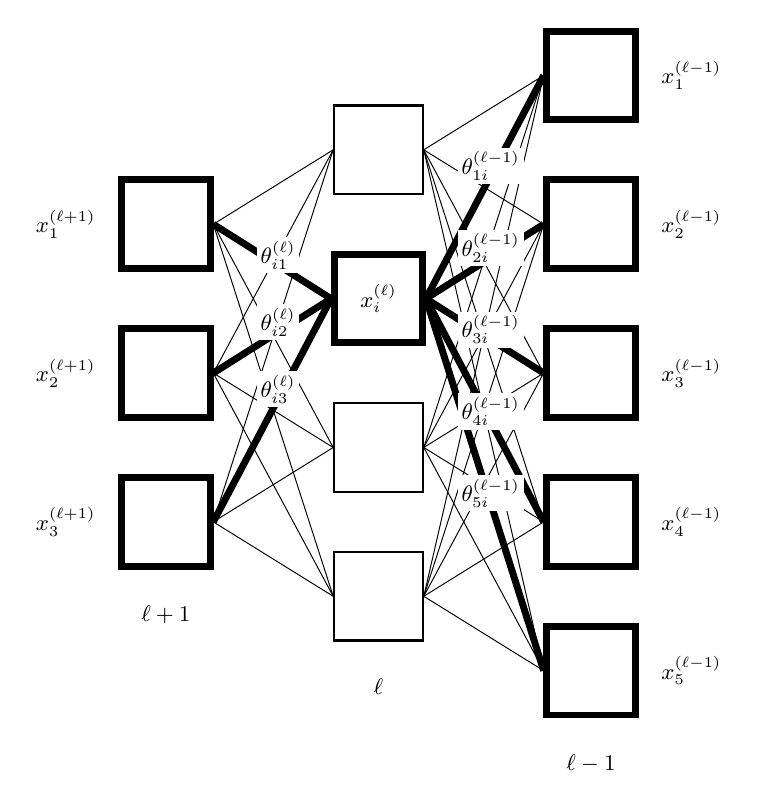
\begin{tikzpicture}[
  scale=0.9, transform shape,
  sq/.style={draw=black, thick, minimum size=1.25cm},
  sqcore/.style={draw=black, line width=2.5pt, minimum size=1.25cm},
  edge/.style={draw=black, line width=0.35pt},
  edgecore/.style={draw=black, line width=2.5pt},
  lab/.style={font=\small},
  thetalab/.style={font=\small, fill=white, inner sep=1.5pt}
]

\def\dy{2.1}
\def\dx{3.0}
\coordinate (C) at (0,0);

\node[sqcore] (L1) at ($(C)+(-\dx,  \dy)$) {};
\node[sqcore] (L2) at ($(C)+(-\dx,   0)$) {};
\node[sqcore] (L3) at ($(C)+(-\dx, -\dy)$) {};

\node[sq]     (M1) at ($(C)+(0, 1.5*\dy)$) {};
\node[sqcore] (M2) at ($(C)+(0, 0.5*\dy)$) {};
\node[sq]     (M3) at ($(C)+(0,-0.5*\dy)$) {};
\node[sq]     (M4) at ($(C)+(0,-1.5*\dy)$) {};

\node[sqcore] (R1) at ($(C)+(\dx,  2*\dy)$) {};
\node[sqcore] (R2) at ($(C)+(\dx,  1*\dy)$) {};
\node[sqcore] (R3) at ($(C)+(\dx,   0)$) {};
\node[sqcore] (R4) at ($(C)+(\dx, -1*\dy)$) {};
\node[sqcore] (R5) at ($(C)+(\dx, -2*\dy)$) {};

\node[lab, left=2mm of L1] {$x^{(\ell+1)}_{1}$};
\node[lab, left=2mm of L2] {$x^{(\ell+1)}_{2}$};
\node[lab, left=2mm of L3] {$x^{(\ell+1)}_{3}$};

\node[lab] at (M2.center) {$x^{(\ell)}_{i}$};

\node[lab, right=2mm of R1] {$x^{(\ell-1)}_{1}$};
\node[lab, right=2mm of R2] {$x^{(\ell-1)}_{2}$};
\node[lab, right=2mm of R3] {$x^{(\ell-1)}_{3}$};
\node[lab, right=2mm of R4] {$x^{(\ell-1)}_{4}$};
\node[lab, right=2mm of R5] {$x^{(\ell-1)}_{5}$};

\foreach \i in {1,2,3} {
  \foreach \j in {1,2,3,4} {
    \draw[edge] (L\i.east) -- (M\j.west);
  }
}
\foreach \i in {1,2,3,4} {
  \foreach \j in {1,2,3,4,5} {
    \draw[edge] (M\i.east) -- (R\j.west);
  }
}

\foreach \j in {1,2,3} {
  \draw[edgecore] (L\j.east) -- (M2.west);
}
\foreach \k in {1,2,3,4,5} {
  \draw[edgecore] (M2.east) -- (R\k.west);
}

\foreach \j in {1,2,3} {
  \node[thetalab] at ($(L\j.east)!0.55!(M2.west)+(0,4pt)$) {$\theta^{(\ell)}_{i\j}$};
}
\foreach \k in {1,2,3,4,5} {
  \node[thetalab] at ($(M2.east)!0.55!(R\k.west)+(0,4pt)$) {$\theta^{(\ell-1)}_{\k i}$};
}

\node[lab, below=4mm of L3] {$\ell + 1$};
\node[lab, below=4mm of M4] {$\ell$};
\node[lab, below=4mm of R5] {$\ell - 1$};

\end{tikzpicture}
\end{center}
\vspace{0.5em}

\subsection{Neural core micro-architecture}
\label{sec:core}

Each neural core contains:
\begin{enumerate}[leftmargin=*]
  \item \textbf{Local state and parameter storage.}
  The core stores its scalar state \( x_i^{(\ell)} \), prediction error \( \varepsilon_i^{(\ell)} \), and a local vector of synaptic weights \( \theta^{(\ell)}_{ij} \), including an explicit bias lane implemented as an additional fixed presynaptic channel. Learning rates \( \alpha \) and activity step size \( \gamma \) are supplied externally but applied locally, with no shared parameter memory.

\item \textbf{Presynaptic activation and gating logic.}
  Presynaptic inputs are communicated between layers as raw state values \(x_j^{(\ell+1)}\). Within the receiving neuron, these values are transformed by an activation \( f(\cdot) \) selected per layer when forming predictions and weight updates. The derivative \( f'(x) \) is computed locally from the neuron's effective state used during the current tick and gates the bottom-up term during the state update. The bias lane is treated as a constant unit feature.

  \item \textbf{Sequential DSP datapath.}
  A single MAC datapath performs prediction accumulation, weight updates, and construction of backpropagated products by iterating over indices, trading throughput for reduced area.

  \item \textbf{Local FSM scheduler.}
  Each core sequences computation through
  \[
    \text{PRED} \rightarrow \text{ERR} \rightarrow \text{BACKSUM} \rightarrow \text{BACKVEC}
    \rightarrow \text{WUP} \rightarrow \text{STATE}.
  \]
  The schedule is identical during inference and learning; whether weights update and whether state values are clamped are controlled externally.

  \item \textbf{Hardwired neighbor interfaces.}
  Each core communicates only:
  \begin{itemize}[leftmargin=*]
    \item its current state \( x_i^{(\ell)} \) downward to layer \( \ell-1 \),
    \item products used to form the bottom-up term upward to layer \( \ell+1 \).
  \end{itemize}
  Communication is point-to-point with no global arbitration.
\end{enumerate}

\subsection{FSM stages}
\label{sec:fsm}

Each tick executes one complete update:
\begin{itemize}[leftmargin=*]
  \item \textbf{PRED}: compute
  \[
  \mu_i^{(\ell)} = \sum_j \theta^{(\ell)}_{ij} f(x_j^{(\ell+1)}),
  \]
  including the explicit bias lane.

  \item \textbf{ERR}: compute and store
  \[
  \varepsilon_i^{(\ell)} = x_{i,\mathrm{eff}}^{(\ell)} - \mu_i^{(\ell)}.
  \]

  \item \textbf{BACKSUM}: accumulate
  \[
  b_i^{(\ell)} = \sum_k \theta^{(\ell-1)}_{k i}\varepsilon_k^{(\ell-1)}
  \]
  from lower-layer signals.

  \item \textbf{BACKVEC}: emit products
  \[
  \theta^{(\ell)}_{ij}\varepsilon_i^{(\ell)}
  \]
  for all non-bias presynaptic indices \(j\), so that the adjacent upper layer can form its bottom-up term.

  \item \textbf{WUP}: update weights
  \[
  \theta^{(\ell)}_{ij} \leftarrow \theta^{(\ell)}_{ij} + \alpha \varepsilon_i^{(\ell)} f(x_j^{(\ell+1)}).
  \]
  In inference-only operation, this stage still executes structurally, but becomes a numerical no-op when \(\alpha = 0\).

  \item \textbf{STATE}: update state using
  \[
  x_i^{(\ell)} \leftarrow x_i^{(\ell)} + \gamma \left( f'\!\left(x_{i,\mathrm{eff}}^{(\ell)}\right) b_i^{(\ell)} - \varepsilon_i^{(\ell)} \right),
  \]
  unless hard clamping overwrites the stored state at the end of the tick.
\end{itemize}

\subsection{Network-level clamping for supervised learning and inference}
\label{sec:clamp}

Each core exposes:
\begin{itemize}[leftmargin=*]
  \item \texttt{x\_set\_en}: enables an externally supplied observation for the current tick,
  \item \texttt{x\_obs}: observed state value.
\end{itemize}

The RTL defines an effective state
\[
x_{i,\mathrm{eff}}^{(\ell)} =
\begin{cases}
x^{(\ell)}_{\mathrm{obs},i} & \text{if } \texttt{x\_set\_en}_i = 1, \\
x_i^{(\ell)} & \text{otherwise},
\end{cases}
\]
which is used during the tick when computing local prediction error and the local derivative gate. The stored state register is then updated at the end of the tick as
\[
x_i^{(\ell)} \leftarrow
\begin{cases}
x^{(\ell)}_{\mathrm{obs},i}
& \text{if } \texttt{CLAMP\_HARD}=1 \ \land\ \texttt{x\_set\_en}_i = 1, \\
x_i^{(\ell)} + \gamma \left( f'\!\left(x_{i,\mathrm{eff}}^{(\ell)}\right)b_i^{(\ell)} - \varepsilon_i^{(\ell)} \right)
& \text{otherwise}.
\end{cases}
\]

Thus, clamping affects not only the final stored state, but also the computation performed during the tick whenever an external observation is present.

Supervised learning clamps boundary layers such as input and target output layers, while inference clamps only the input and reads the free output after a fixed tick budget.

\subsection{Tick-based execution model}

Computation proceeds in discrete ticks controlled by an external clock.
Each tick triggers a full execution of the neural-core finite-state schedule.
At the network level, a global \texttt{start\_tick} request is converted into
an internal start pulse once the network is idle, and this pulse is then
broadcast to all layer modules and neural cores.

Each core asserts a \texttt{done} signal upon completion of its local update.
Layer modules latch per-core completion and emit a one-shot layer-level done
pulse once all neurons in the layer have completed. The network module applies
the same aggregation strategy across layers and emits a one-shot network-level
\texttt{done} pulse once all layers have completed the current tick.

This organization yields a deterministic tick schedule without requiring any
asynchronous coordination inside the neural cores themselves.

From a dynamical-systems perspective, each tick corresponds to one explicit
Euler-style step of the predictive-coding dynamics described in
Section~\ref{sec:pc-discrete}.

\section{Implementation Details}
\label{sec:impl}

\subsection{Arithmetic format}
All arithmetic is performed in IEEE-754 single precision using HardFloat recoded format (recFN). Rounding mode is fixed to round-to-nearest-even. Multiply, add, and fused multiply-add units are reused sequentially across indices.

\subsection{Sequential datapath}
Each core iterates across presynaptic indices during prediction and weight update stages. As a result, the cycle count per tick scales linearly with fan-in. This design choice trades throughput for reduced area and a uniform per-core implementation.

\subsection{Bias lane}
A bias lane is implemented as an additional presynaptic feature with constant value \(1\). The bias weight can optionally use an independent learning-rate scale or be frozen.

\subsection{Hardware cost model}

Because each neural core reuses a sequential multiply--accumulate datapath,
the cycle count per tick scales linearly with fan-in.

Let \(N\) denote the number of true presynaptic inputs and \(M\) the number of
backpropagated error inputs. The implemented FSM executes:
\begin{itemize}[leftmargin=*]
\item \(N+1\) cycles for prediction accumulation, including the explicit bias lane,
\item \(1\) cycle for error formation,
\item \(M\) cycles for accumulation of lower-layer back inputs,
\item \(N\) cycles to emit the upward back vector,
\item \(N+1\) cycles for weight updates, again including the bias lane,
\item \(1\) cycle for the state update.
\end{itemize}

Accordingly, the per-tick cycle count is approximately
\[
C_{\text{tick}} = (N+1) + 1 + M + N + (N+1) + 1 = 3N + M + 4.
\]

Thus the design has \emph{linear tick latency} in both presynaptic fan-in and incoming
back-error fan-in. This sequential organization reduces area per neuron but
increases latency per tick. Higher-throughput implementations could introduce
parallel MAC units or vectorized datapaths.

\section{Stability and Convergence Considerations}
\label{sec:stability}

Predictive coding is often presented as gradient descent on a prediction-error energy in continuous time \cite{friston2005theory}. The hardware described here implements a discrete-time variant with finite precision, a fixed per-tick computation schedule, optional clamping, and simultaneous activity and weight updates. These departures matter: stability properties of idealized continuous-time dynamics do not automatically transfer to a tick-based explicit Euler discretization in floating-point arithmetic.

Accordingly, we treat stability in this work as an empirical property to be characterized as a function of step sizes, initialization, activation choice, and tick budget.

\subsection{Relation to backpropagation and incremental predictive coding}
Predictive coding can approximate backpropagation-like error signals under converged inference and standard modeling assumptions \cite{Whittington2017}. The present system does not assume inference convergence between parameter updates, and instead operates in an incremental regime with a fixed number of ticks per example. Recent analyses of incremental predictive coding motivate such schedules and connect them to incremental EM viewpoints \cite{salvatori2023stable, neal1998view, karimi2019global}, but do not directly guarantee stability for a particular hardware discretization.

\section{Experiments}
\label{sec:experiments}

The first two experiments (Sections~\ref{sec:exp-function}--\ref{sec:exp-tanh})
are implemented as Verilator simulations using the reference RTL implementation.
The scaling experiment (Section~\ref{sec:exp-scaling}) and the remaining
characterisation experiments use the \texttt{python\_rtl} floating-point
reference implementation, whose agreement with RTL float32 arithmetic is
formally bounded in Section~\ref{sec:exp-fidelity}.

\subsection{Teacher--student regression}
\label{sec:exp-function}

A three-layer network (\(2 \rightarrow 4 \rightarrow 3\)) with a ReLU hidden
layer is trained to match a fixed teacher \(y = A_{\mathrm{gt}}\,
\mathrm{ReLU}(B_{\mathrm{gt}} x)\). Input and output layers are clamped;
the hidden layer is free. MSE begins at \(0.341207\), spikes briefly to
\(0.369199\) at epoch \(1\), then descends rapidly to \(0.004784\) by
epoch \(7\) before settling to \(0.005935\) at epoch \(25\)
(Figure~\ref{fig:relu_training}). The two-phase profile --- sharp initial
descent followed by a slow plateau --- is consistent with the incremental
tick regime, in which inference does not fully converge between weight updates.

\begin{figure}[H]
\centering
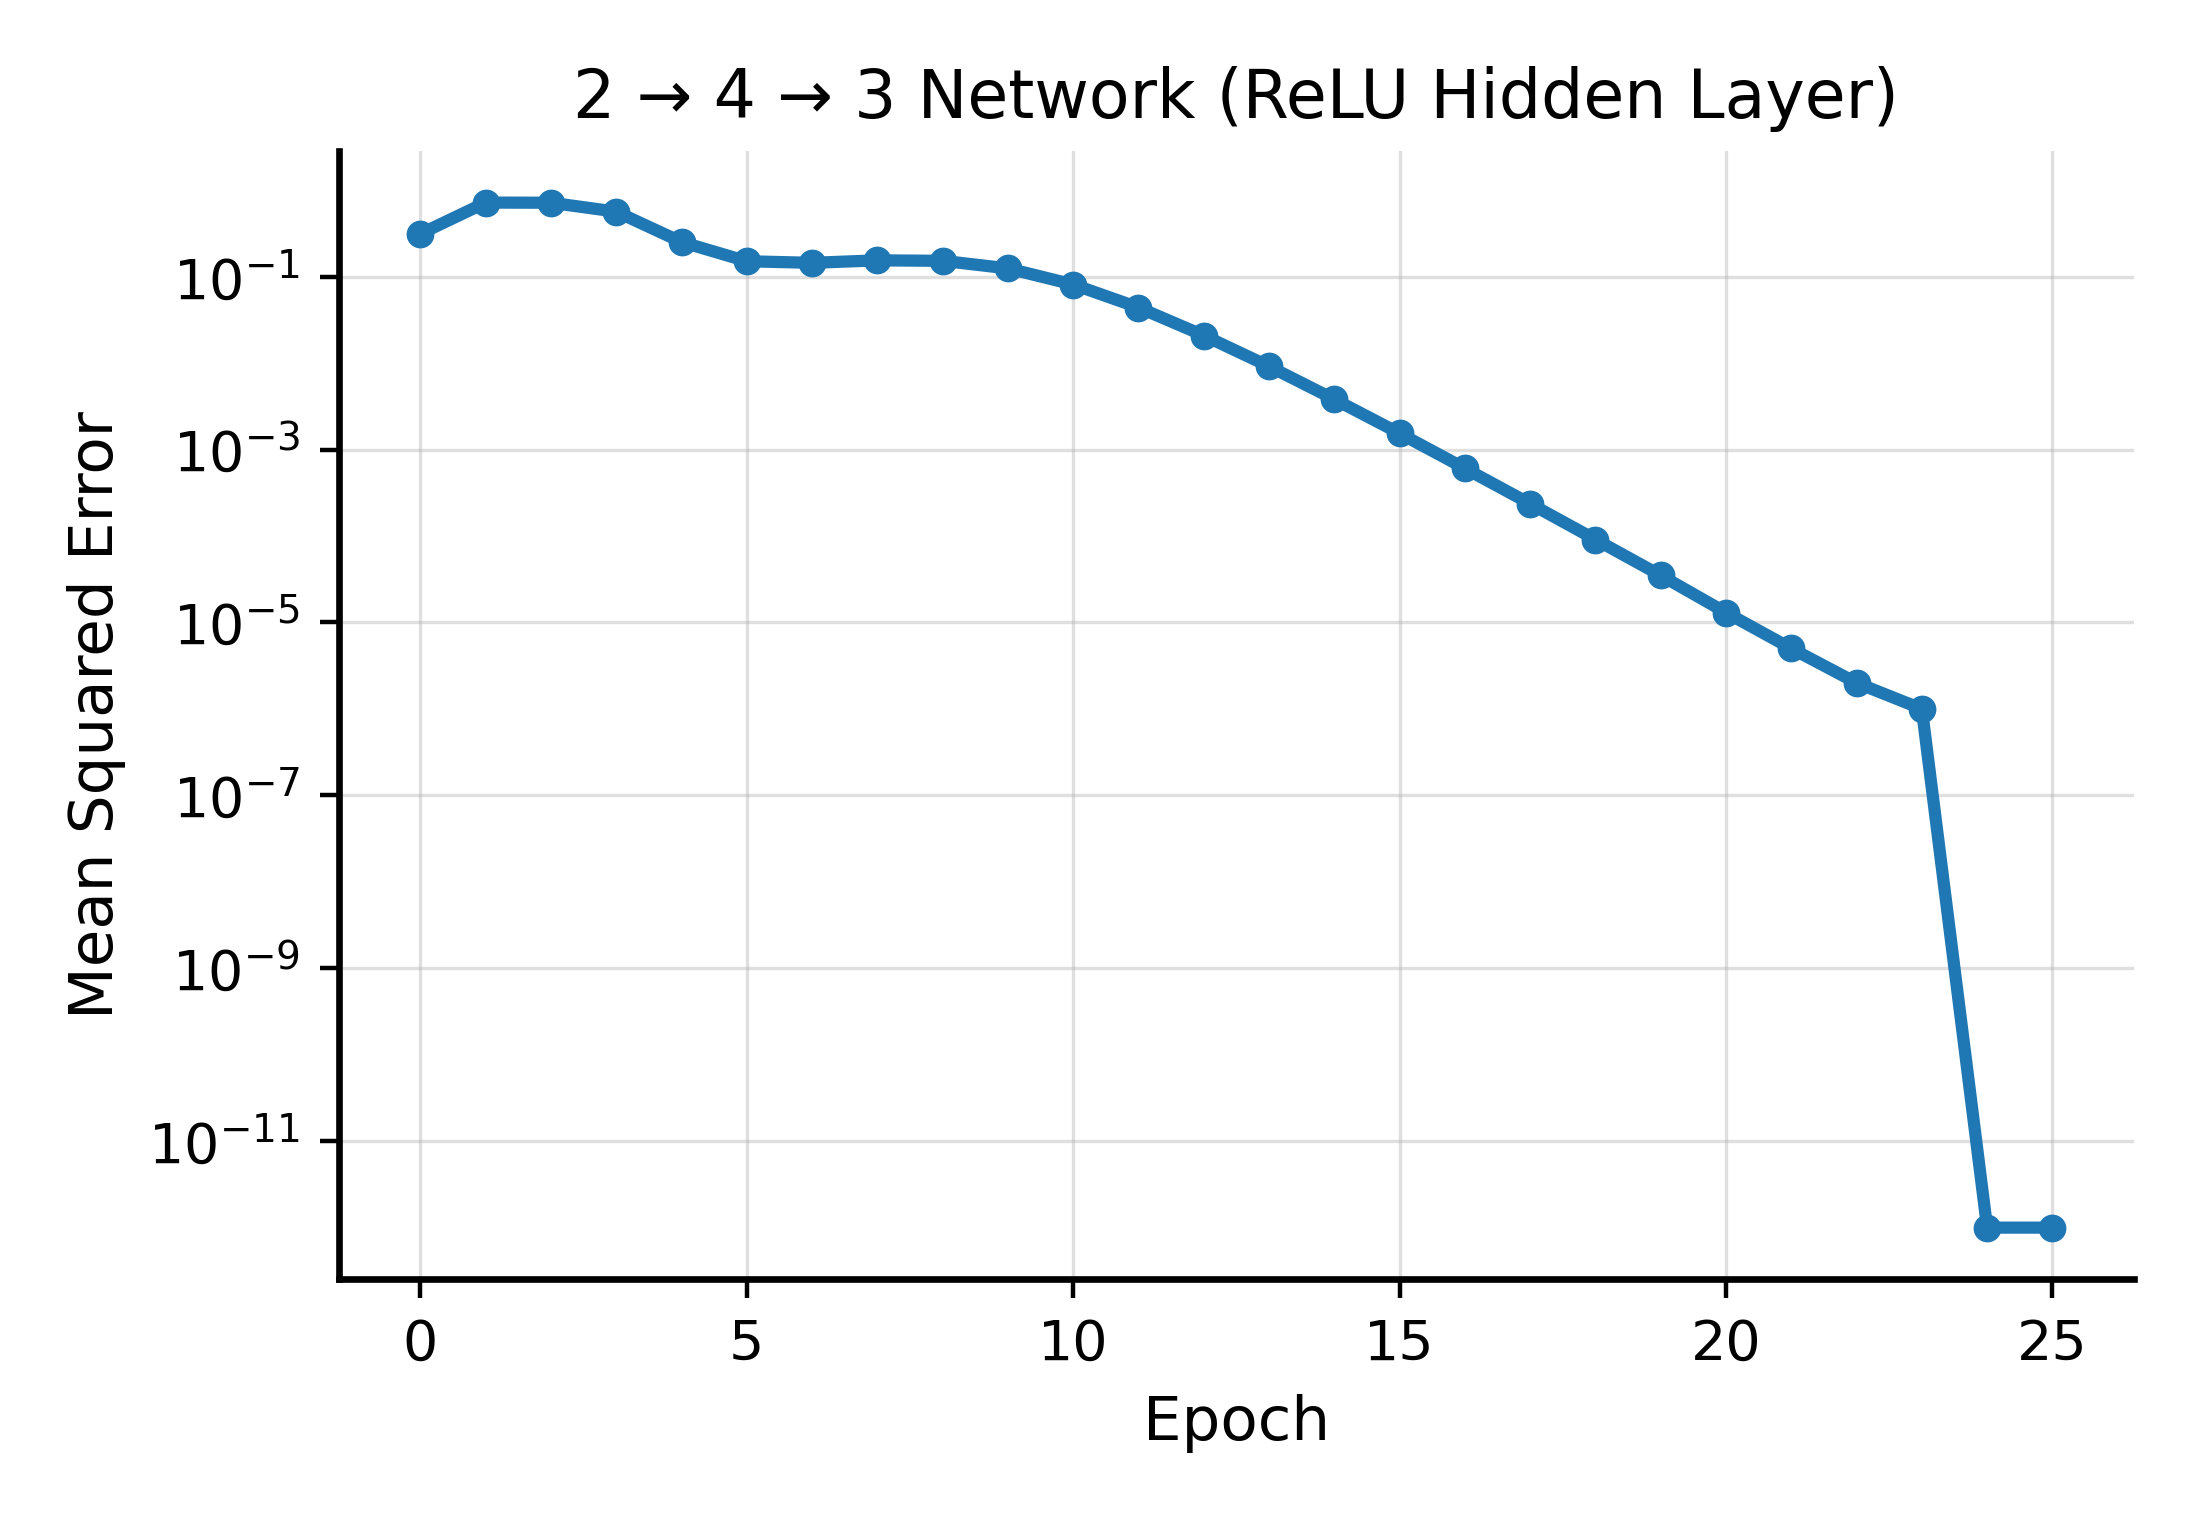
\includegraphics[width=0.75\linewidth]{figures/relu_training_curve.png}
\caption{Training curve for the \(2 \rightarrow 4 \rightarrow 3\) ReLU
network. After a brief transient at epoch \(1\), MSE descends rapidly then
settles into a slow-improvement plateau.}
\label{fig:relu_training}
\end{figure}

\subsection{Nonlinear regression with hidden tanh layer}
\label{sec:exp-tanh}

A smaller network (\(2 \rightarrow 2 \rightarrow 1\)) with a tanh hidden layer
is trained on targets \(y = A_{\mathrm{gt}} \tanh(B_{\mathrm{gt}} x + b_1)
+ b_2\). MSE begins at \(1.106512\), spikes to \(1.986610\) at epoch \(1\),
then collapses to \(0.004725\) by epoch \(3\) --- a reduction of more than
two orders of magnitude in two epochs. Subsequent improvement is slow and
monotone, reaching \(0.004382\) at epoch \(25\)
(Figure~\ref{fig:tanh_training}).

\begin{figure}[H]
\centering
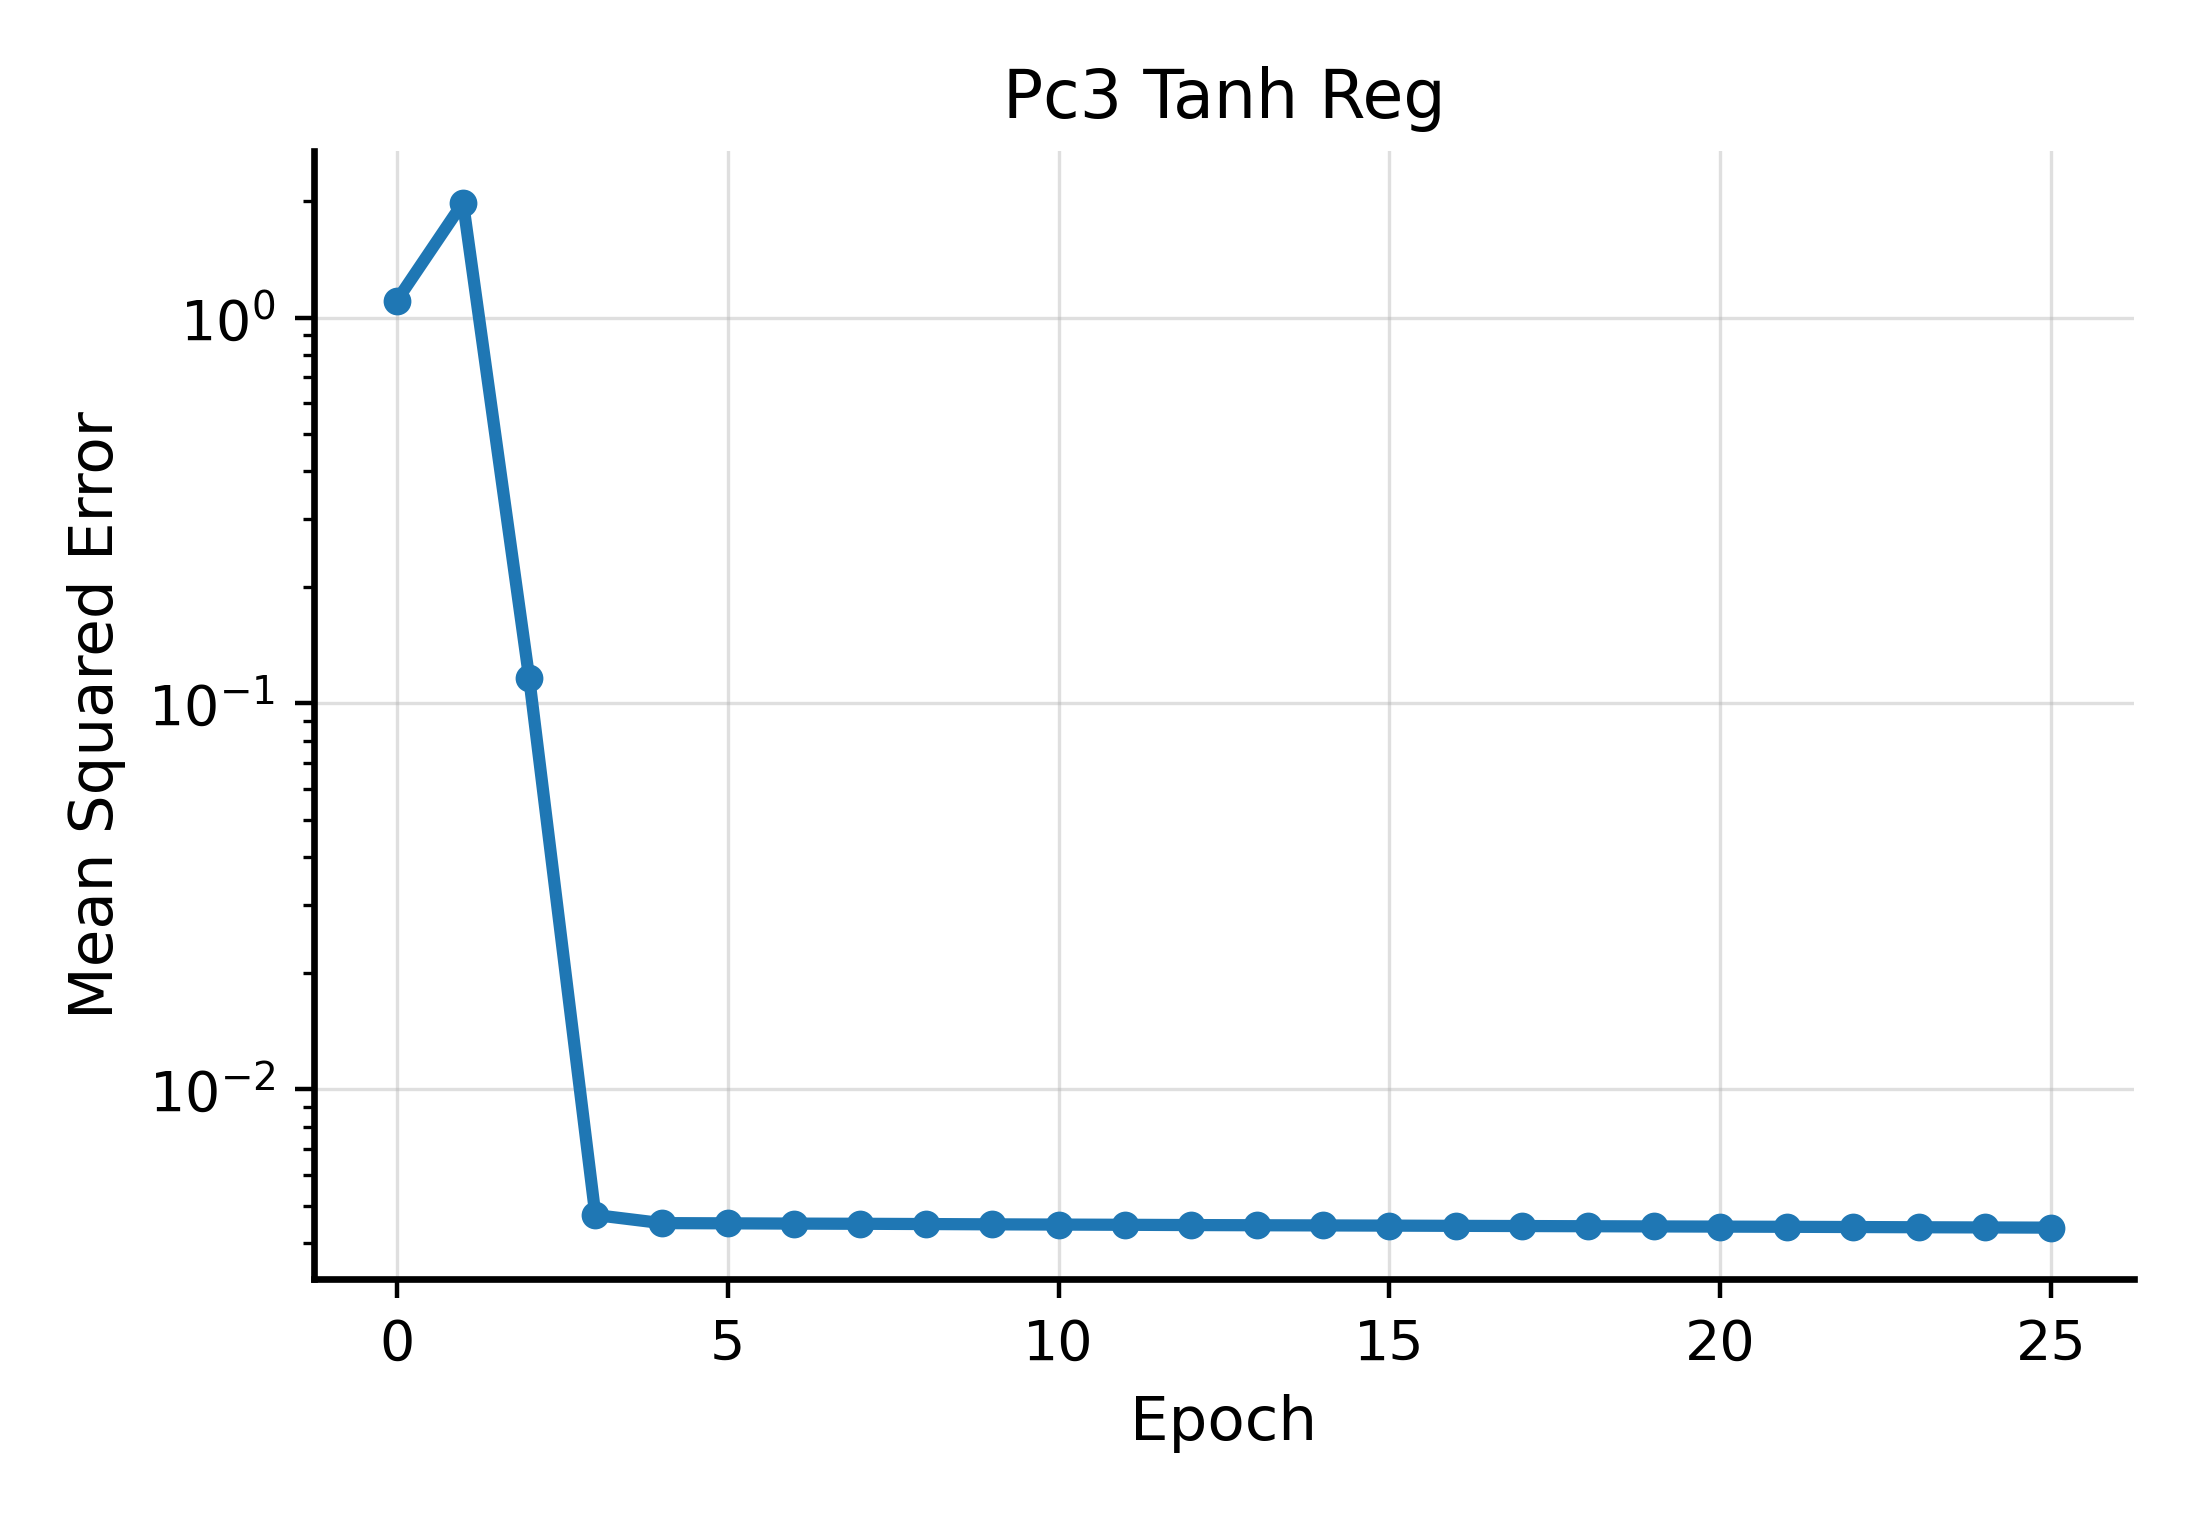
\includegraphics[width=0.75\linewidth]{figures/tanh_training_curve.png}
\caption{Training curve for the \(2 \rightarrow 2 \rightarrow 1\) tanh
network. MSE drops more than two orders of magnitude by epoch \(3\) and
subsequently improves slowly to a small residual.}
\label{fig:tanh_training}
\end{figure}

\subsection{Architectural scaling}
\label{sec:exp-scaling}

To test whether the local update dynamics generalise across network sizes,
the same tick schedule, clamping interface, and training protocol are applied
to three architectures using a single parameterised testbench
(\texttt{tb\_scale\_function.py}):
\[
2 \rightarrow 4 \rightarrow 3, \quad
4 \rightarrow 8 \rightarrow 4, \quad
8 \rightarrow 16 \rightarrow 8.
\]
No changes are made to the neural-core FSM or clamping logic; only the
compile-time dimension parameters differ.

\paragraph{Teacher and activation.}
All three configurations use a \emph{sparse tiled tanh} teacher
\[
y = A \cdot \tanh\!\left(B \cdot \tanh(x)\right),
\]
where $B \in \mathbb{R}^{K_1 \times K_2}$ is a sparse weight matrix with at
most two nonzero entries per row, constructed from a fixed four-row motif
tiled across hidden units, and $A \in \mathbb{R}^{K_0 \times K_1}$ is a
sparse readout tiled from a three-row motif.  The student network uses
$f = \tanh$ in both the hidden and bottom layers, matching the teacher's
function class exactly so that zero training error is achievable in principle.
Biases are included as a fixed presynaptic lane in the hidden layer.

\paragraph{Curse of dimensionality and the role of sparse structure.}
The choice of a structurally sparse teacher is not arbitrary: it is required
for reliable convergence under a fixed sample budget as input dimension grows.
A dense random teacher of the form $y = W_2 \tanh(W_1 \tanh(x) + b)$ ---
with $W_1 \in \mathbb{R}^{K_1 \times K_2}$ fully dense --- produces a function
that varies across all $K_2$ input dimensions simultaneously.  By the curse of
dimensionality, the number of training samples needed to cover the input space
at resolution $\varepsilon$ scales as $O((1/\varepsilon)^{K_2})$: for $K_2=8$
and a coarse resolution of $\varepsilon=0.2$ this already exceeds $10^5$, making
a fixed budget of a few hundred samples hopelessly sparse.

Beyond coverage, dense teachers also create co-adaptation traps during learning.
The two weight matrices $W_1$ (hidden projection) and $W_0$ (output projection)
must be jointly optimized; if one matrix grows fast and locks the hidden
representation into a subspace misaligned with the other, the system stagnates
regardless of sample count or step size.  Empirically, the dense random teacher
plateaus at $\mathrm{MSE} \approx 0.01$ for the $8 \rightarrow 16 \rightarrow
8$ configuration regardless of learning rate or training length.

The sparse tiled teacher sidesteps both issues.  Because $B$ has at most two
nonzero entries per row, each hidden unit effectively depends on a
two-dimensional subspace of the input regardless of $K_2$.  The coverage
problem collapses from $O((1/\varepsilon)^{K_2})$ to $O((1/\varepsilon)^2)$
per unit, and a grid of $2^{K_2}$ to $4^{K_2/2}$ samples provides adequate
coverage at all tested sizes.  The credit-assignment path is also well
conditioned from initialisation: each output unit interacts with a small,
identifiable subset of hidden units rather than a dense superposition of all of
them.

\paragraph{Dataset and training protocol.}
Each configuration is trained on a Cartesian grid of input--output pairs,
with $6^2 = 36$ samples for $K_2=2$ and $2^{K_2}=256$ samples for $K_2 \in
\{4,8\}$, drawn from per-dimension ranges $[-1.2,\,1.2]$ for the first input
dimension, $[-1.1,\,1.1]$ for the second, and shrinking symmetrically for
higher dimensions ($[-1.0,\,1.0]$, $[-0.9,\,0.9]$, \ldots).  The same fixed
random seed is used across all three configurations.  Learning-rate parameters
are $\alpha=0.01$ with multiplicative decay $0.95$ per epoch and
$\gamma=0.04$.

\paragraph{Results.}
All three architectures converge cleanly and monotonically
(Figure~\ref{fig:scaling}). MSE drops more than two orders of magnitude within
the first two epochs across all sizes: from $0.189$ to $0.0035$ for
$2\rightarrow4\rightarrow3$, from $0.218$ to $0.0028$ for
$4\rightarrow8\rightarrow4$, and from $0.282$ to $0.00052$ for
$8\rightarrow16\rightarrow8$.  Final MSE at epoch 25 is $3.8\times10^{-4}$,
$6.3\times10^{-4}$, and $2.2\times10^{-4}$ respectively, with no divergence
or oscillation observed at any scale.  Notably, the largest configuration
achieves the lowest absolute residual, consistent with increasing network
capacity relative to a fixed-complexity sparse teacher.

\begin{figure}[H]
\centering
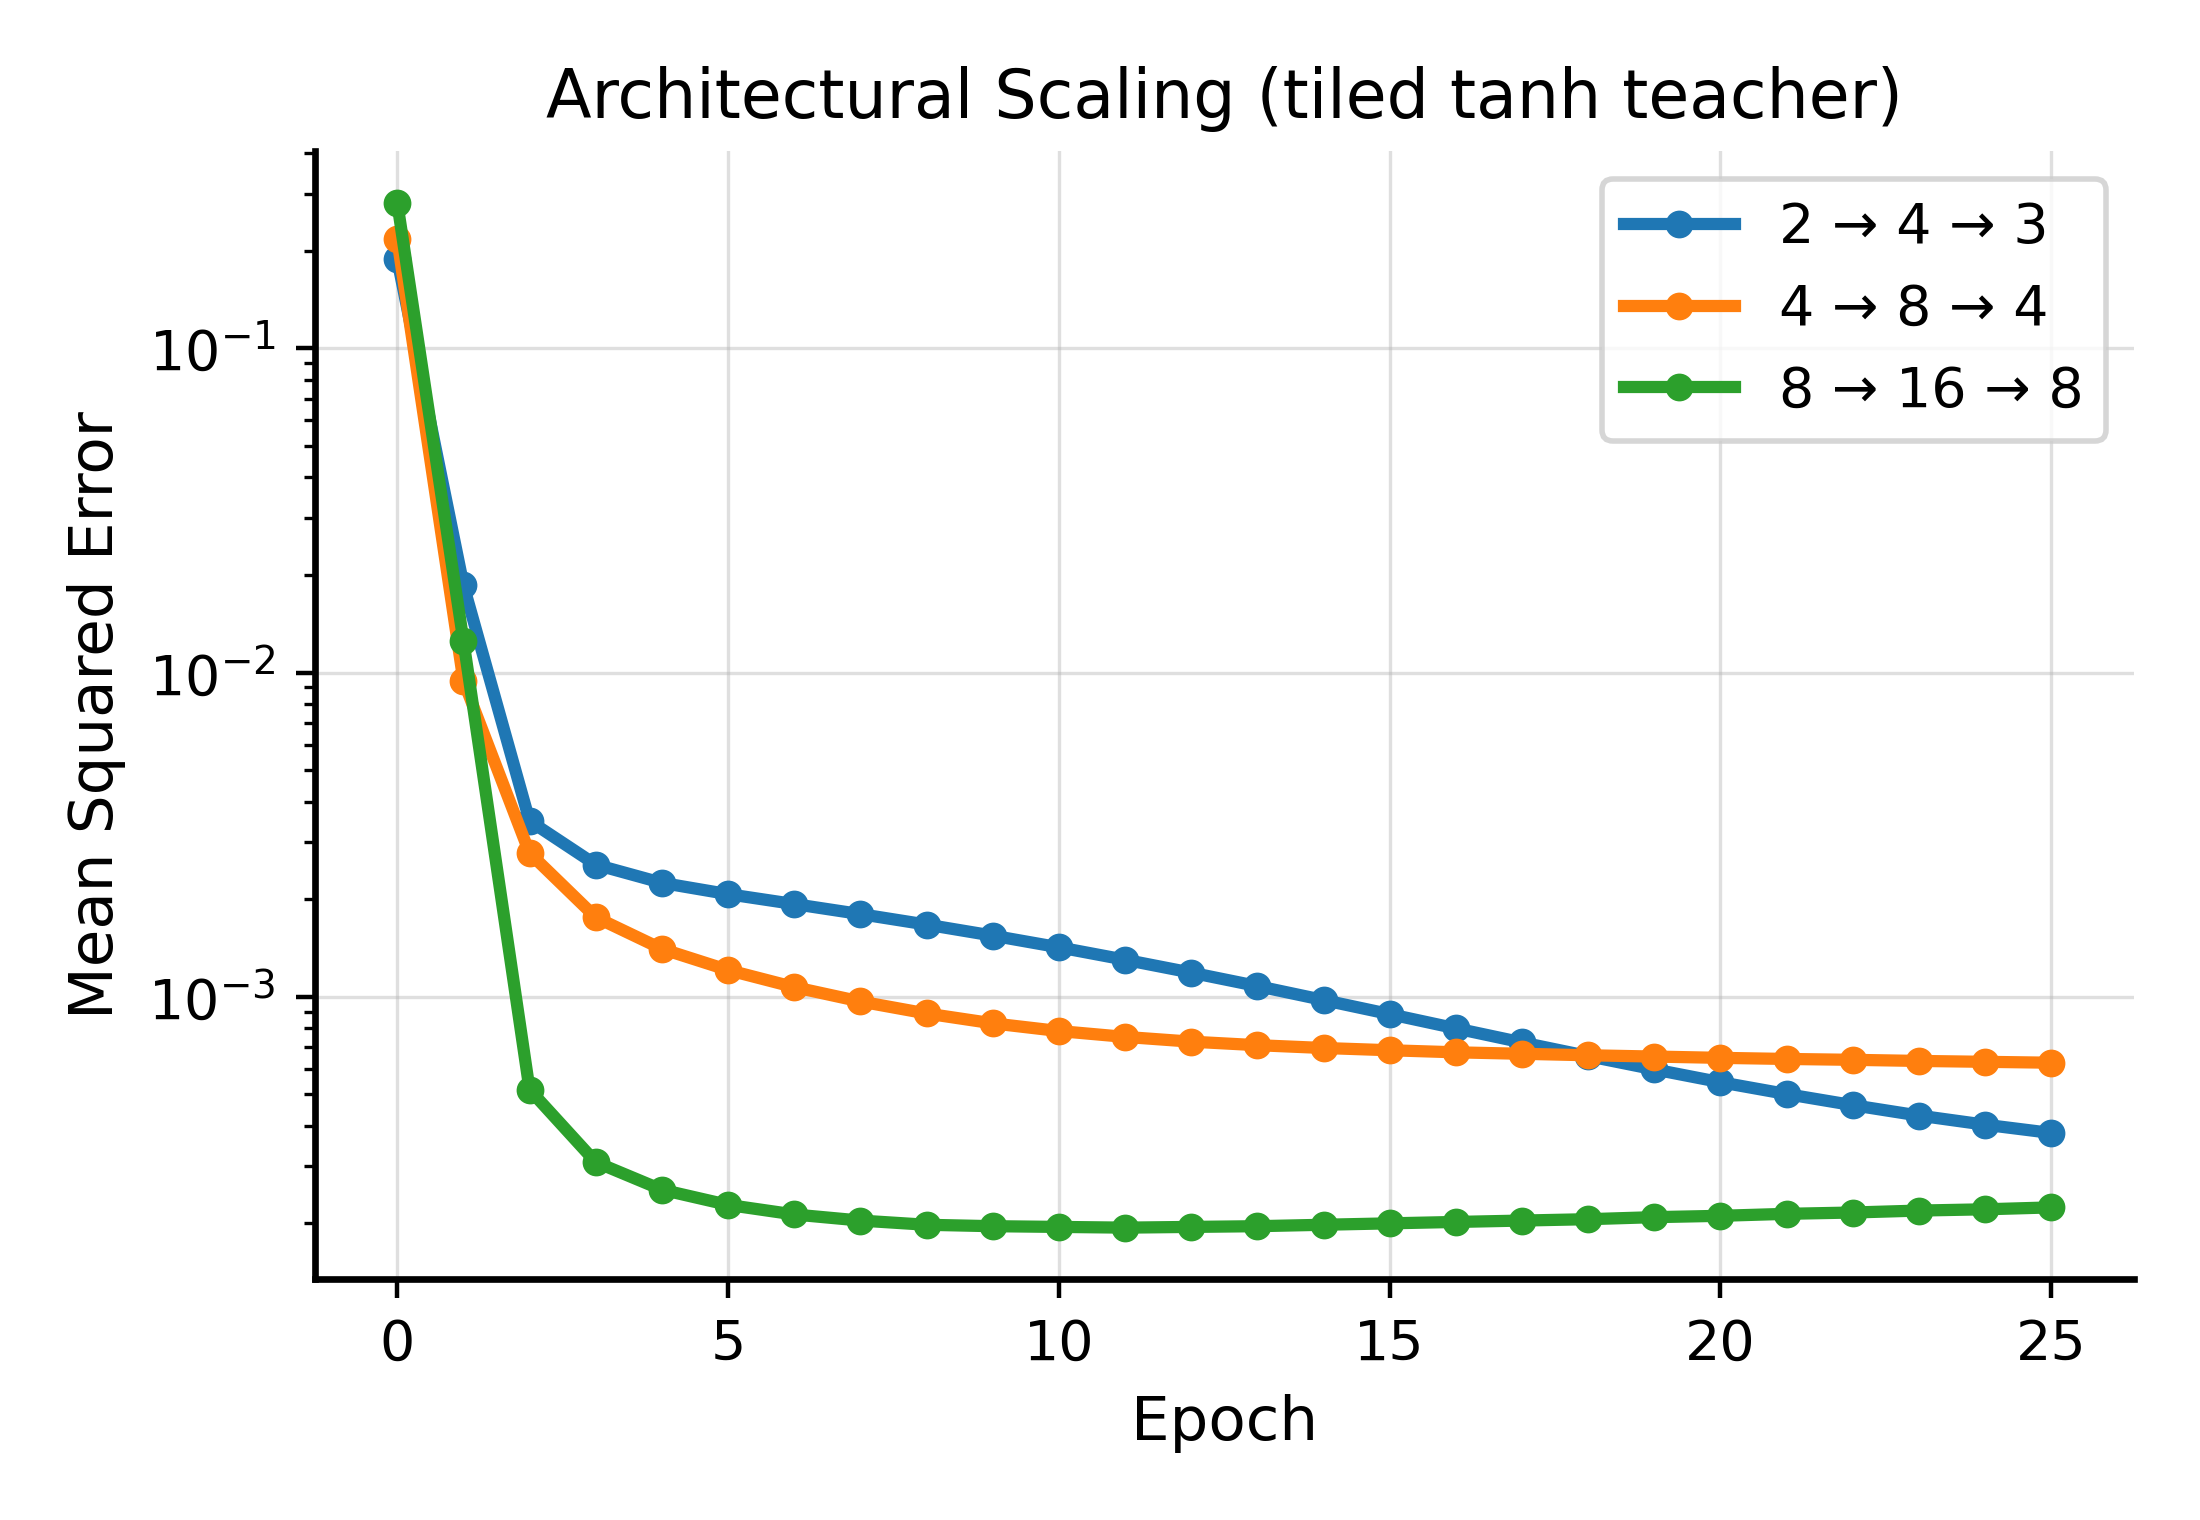
\includegraphics[width=0.75\linewidth]{figures/tanh_scaling.png}
\caption{Training curves for three architectures of increasing dimension,
trained on a Cartesian grid with a sparse tiled tanh teacher
$y = A \cdot \tanh(B \cdot \tanh(x))$.  All three configurations converge
cleanly without oscillation; the largest ($8 \rightarrow 16 \rightarrow 8$)
achieves the lowest absolute residual, consistent with overcomplete
hidden capacity relative to the sparse teacher.}
\label{fig:scaling}
\end{figure}

\subsection{Scaling with random bias initialisation}
\label{sec:exp-scaling-bias}

The previous scaling experiment initialised all bias weights to zero.  To test
whether the local learning dynamics remain effective when biases carry an initial
offset, the same three architectures are retrained under the same protocol
(\(\alpha = 0.01\), decay \(0.95\), \(\gamma = 0.04\), 25~epochs, sparse tiled
tanh teacher) with bias weights drawn from \(\mathcal{N}(0,\,0.5^2)\) at
initialisation (\texttt{--bias-init-scale 0.5}).

\paragraph{Results.}
Random bias initialisation raises the initial MSE across all three
configurations: from $0.189$ to $0.452$ for $2\rightarrow4\rightarrow3$,
from $0.218$ to $0.380$ for $4\rightarrow8\rightarrow4$, and from $0.282$ to
$0.477$ for $8\rightarrow16\rightarrow8$.  Despite this elevated starting
point, all three networks converge to small residuals by epoch~25: $5.0\times
10^{-4}$, $5.2\times10^{-4}$, and $2.3\times10^{-4}$ respectively
(Figure~\ref{fig:scaling_bias}).  The two smaller configurations follow a
convergence profile similar to the zero-bias case, with most of the MSE
reduction occurring in the first two epochs.  The largest configuration
($8\rightarrow16\rightarrow8$) takes more epochs to absorb the initial bias
offset --- dropping below $10^{-3}$ around epoch~4 rather than epoch~2 ---
but still converges cleanly and monotonically.  Final residuals are comparable
to those obtained with zero initialisation, confirming that the local
predictive-coding update rule can absorb non-zero bias initialisation without
any manual tuning of the bias learning rate.

\begin{figure}[H]
\centering
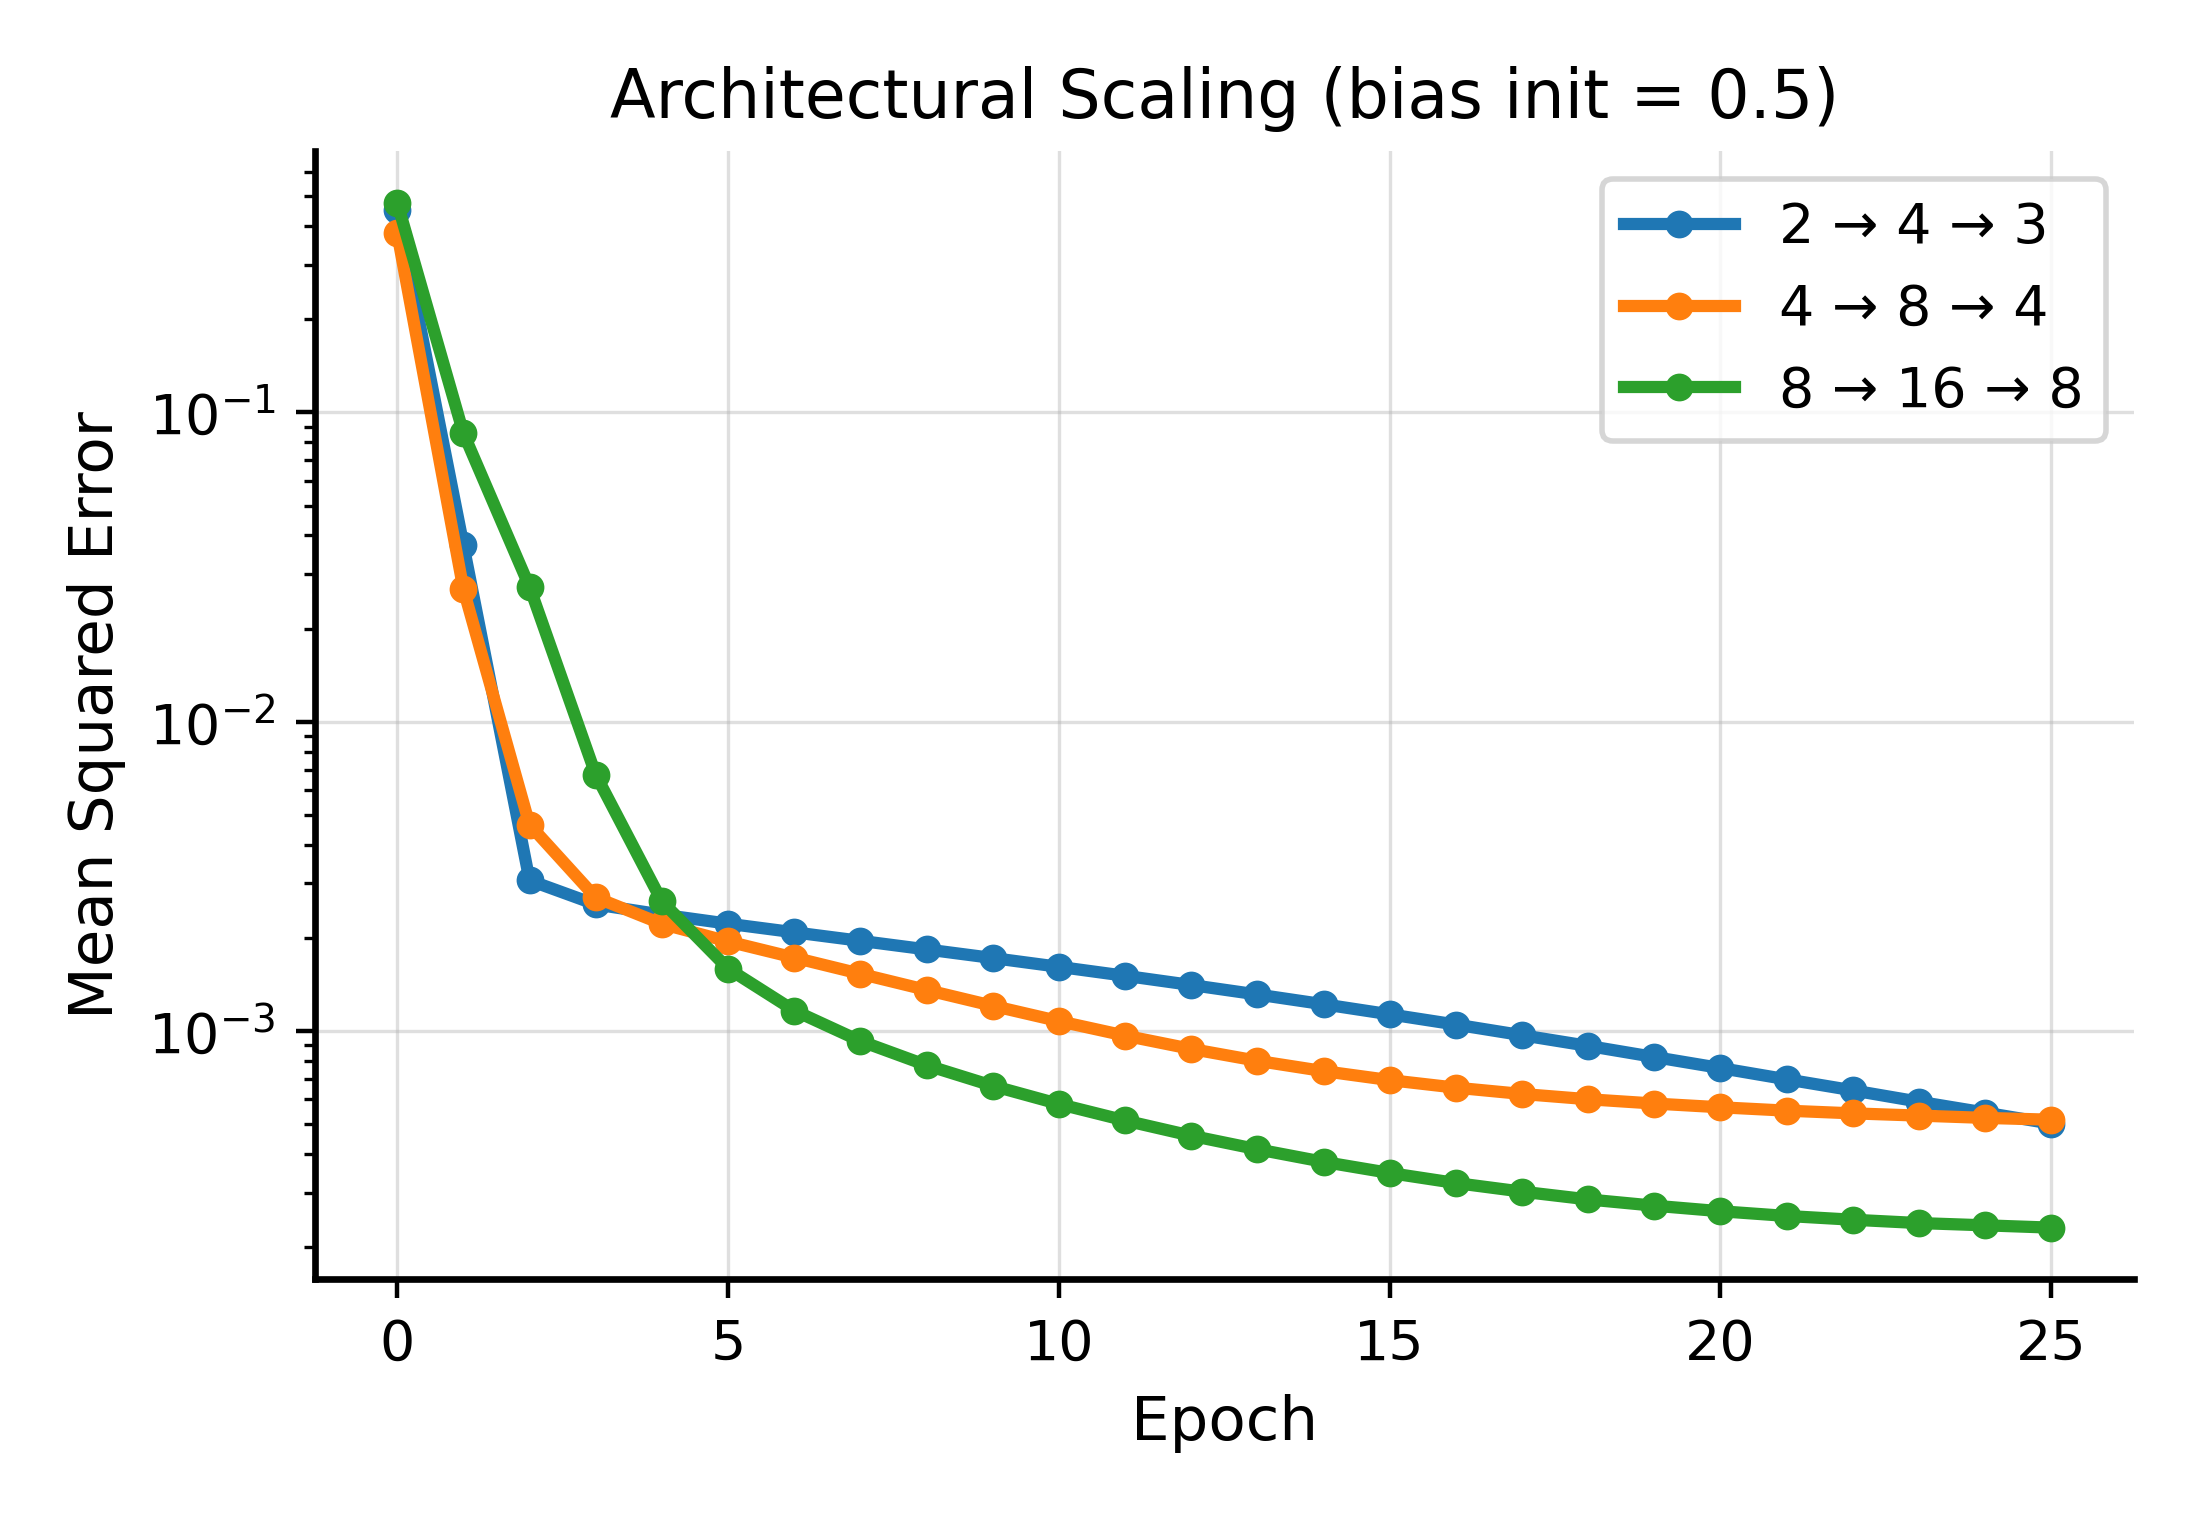
\includegraphics[width=0.75\linewidth]{figures/tanh_scaling_bias.png}
\caption{Training curves for the same three architectures as
Figure~\ref{fig:scaling}, with bias weights initialised from
$\mathcal{N}(0,\,0.5^2)$.  All three configurations converge to comparable
final residuals despite the elevated initial MSE caused by the random bias
offsets; the largest architecture takes a few extra epochs to absorb the
initial offset before descending steeply.}
\label{fig:scaling_bias}
\end{figure}

\subsection{Stability and hyperparameter characterization}
\label{sec:exp-stability}

Section~\ref{sec:stability} claims that stability is treated as an empirical
property to be characterized as a function of step sizes and tick budget.
This subsection delivers that characterization using the Python reference
implementation.

\paragraph{Phase diagram.}
A grid sweep over \(8 \times 8\) \((\alpha, \gamma)\) pairs was conducted on
the \(2 \rightarrow 4 \rightarrow 3\) architecture for 15 epochs, with
\(\alpha \in \{0.001, 0.003, 0.01, 0.03, 0.05, 0.10, 0.15, 0.20\}\) and
\(\gamma \in \{0.005, 0.010, 0.02, 0.04, 0.07, 0.10, 0.15, 0.20\}\).
Each of the 64 grid points is classified as \emph{converged} (final
MSE~$< 0.01$), \emph{stagnated}, \emph{oscillating}, or \emph{diverged}
(Figure~\ref{fig:phase_diagram}).

No run diverged or oscillated across the entire tested range.
Convergence requires approximately \(\gamma \geq 0.07\) regardless of~\(\alpha\):
for all tested learning rates, lowering the inference step size below this
threshold leaves the network stagnated, while raising it above this threshold
yields convergence across the full range of \(\alpha\) values tested.
The paper default \((\alpha=0.01,\,\gamma=0.04)\) falls in the stagnated region
under the 15-epoch budget used here; the tick-budget sweep below shows that
additional inference ticks at this operating point do achieve convergence.

\begin{figure}[H]
\centering
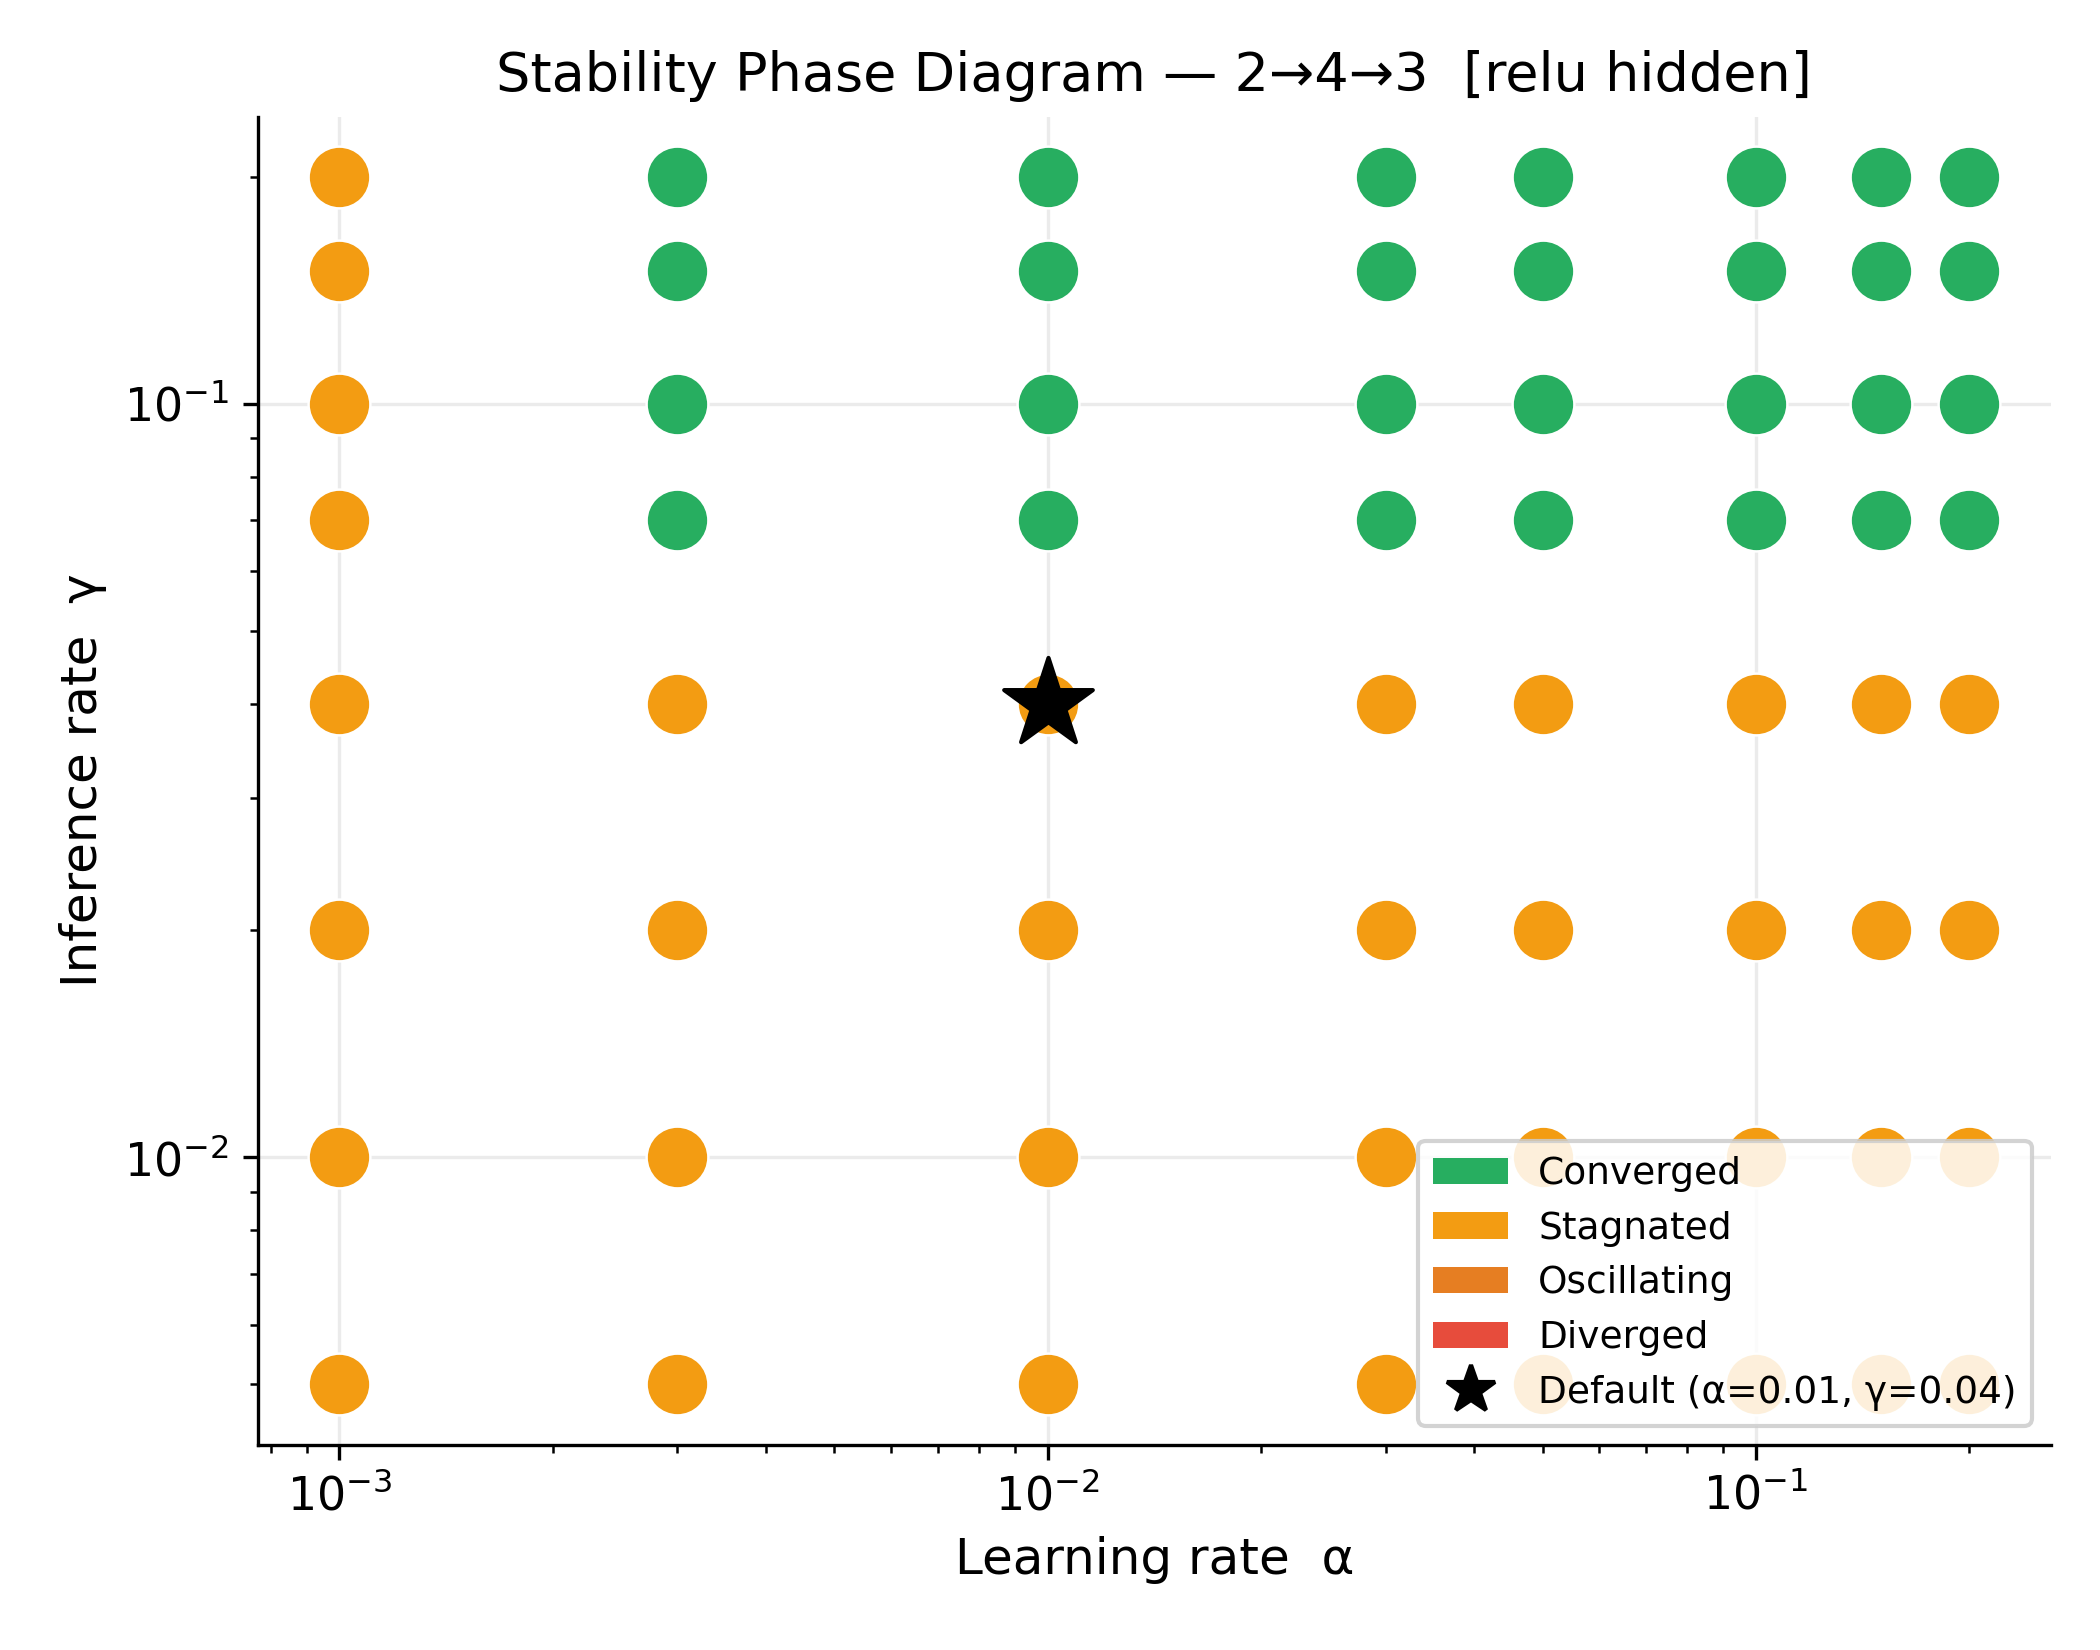
\includegraphics[width=0.75\linewidth]{figures/stability_phase_2x4x3_relu.png}
\caption{Stability phase diagram for the \(2 \rightarrow 4 \rightarrow 3\)
architecture over a \(8 \times 8\) grid of \((\alpha, \gamma)\) pairs.
All 64 points are either converged (green) or stagnated (orange).}
\label{fig:phase_diagram}
\end{figure}

\paragraph{Tick-budget sweep.}
A separate sweep fixes \((\alpha,\gamma) = (0.01, 0.04)\) and varies the
per-sample inference tick budget \(T \in \{1,2,5,10,20,50,100,200,500\}\)
over 20 epochs (Figure~\ref{fig:tick_budget}). Results confirm the incremental
regime claim: at \(T=1\) the network barely improves (MSE $= 0.149$), and each
doubling of \(T\) yields substantial MSE reduction up to \(T \approx 50\)
(MSE $= 0.0077$), after which gains become negligible (\(< 0.1\%\) relative
reduction from \(T=50\) to \(T=500\)). The inference step size \(\gamma\) and
tick budget jointly determine how closely the network equilibrates between
weight updates; the diminishing-returns knee at \(T \approx 50\) identifies a
practical operating point for this architecture.

\begin{figure}[H]
\centering
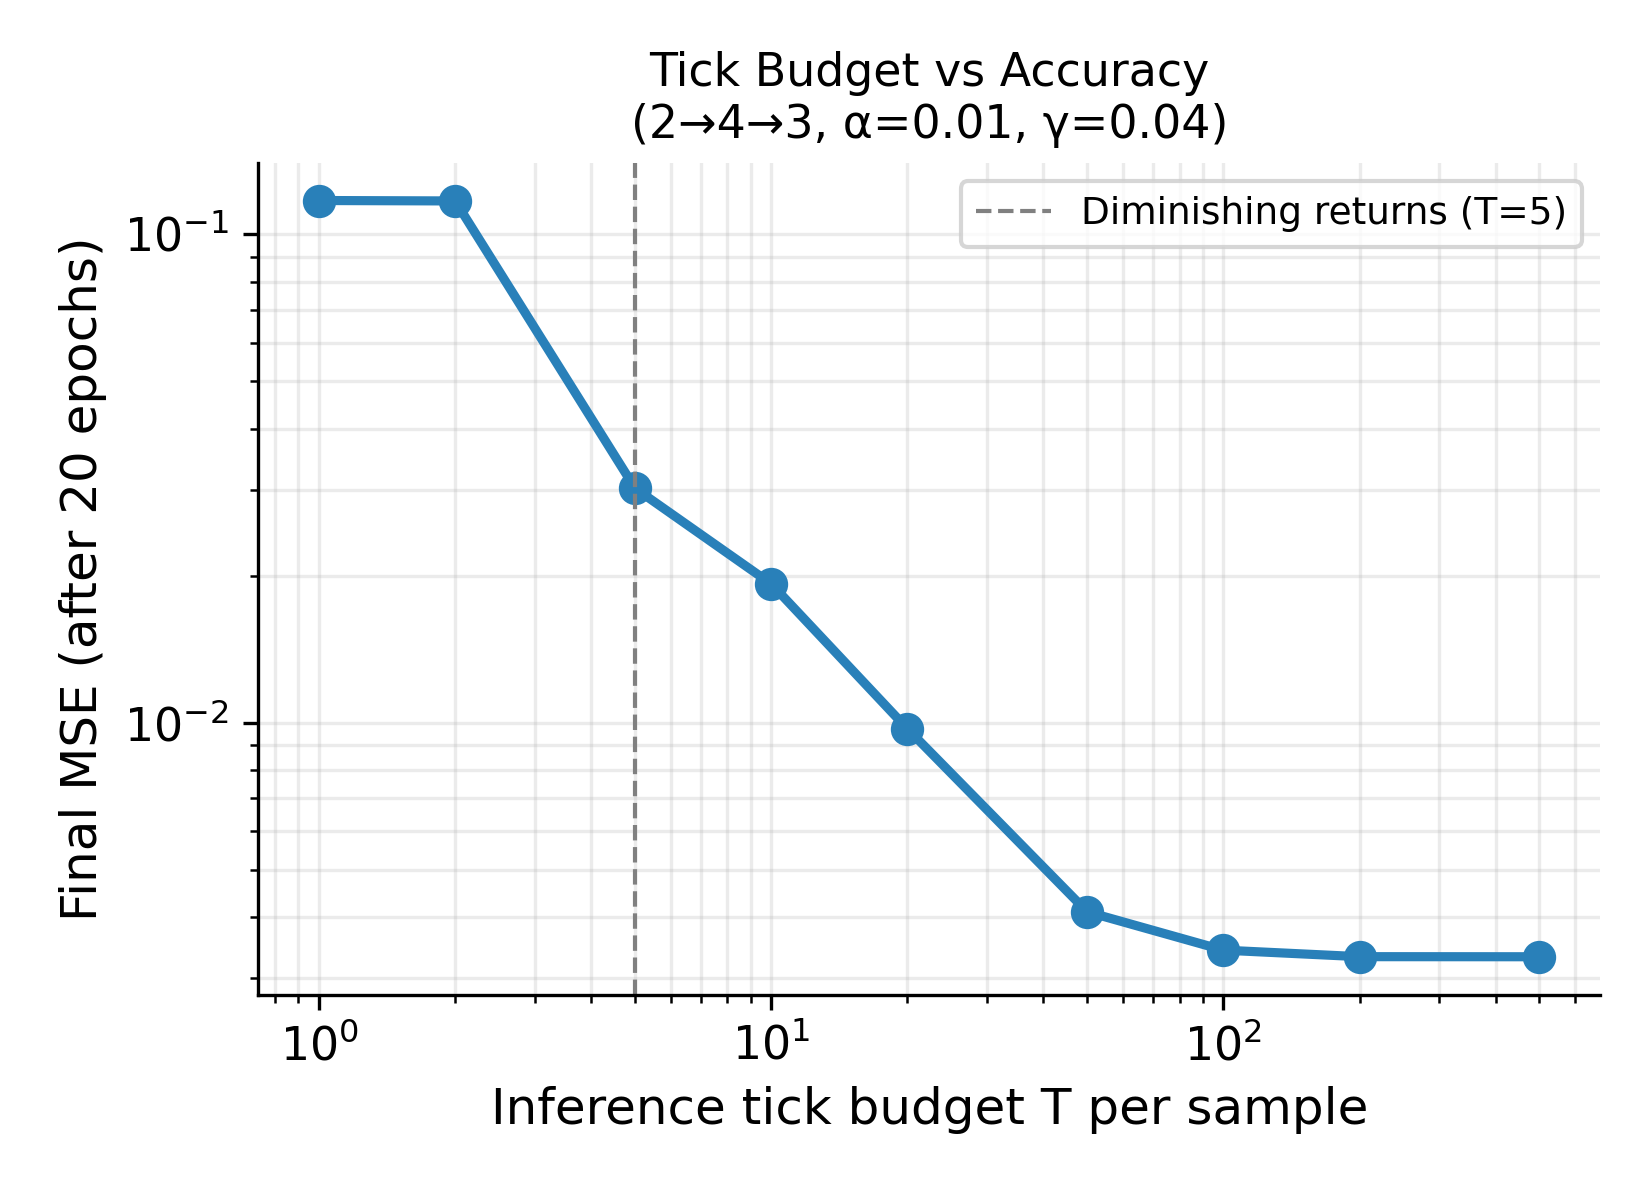
\includegraphics[width=0.65\linewidth]{figures/tick_budget_2x4x3_relu.png}
\caption{Final MSE after 20 epochs as a function of inference tick budget \(T\)
per sample, at fixed \(\alpha=0.01\), \(\gamma=0.04\).
MSE falls from \(0.149\) at \(T=1\) to \(0.0077\) at \(T=50\) and plateaus
thereafter, identifying a practical diminishing-returns knee.}
\label{fig:tick_budget}
\end{figure}

\subsection{Online learning comparison}
\label{sec:exp-online}

To contextualize the PC network's learning efficiency, a backpropagation MLP
with identical topology (\(2 \rightarrow 4 \rightarrow 3\), ReLU hidden layer)
and matched weight initialization is trained in the strictly online regime:
each of 3000 training samples is presented exactly once, with no replay or
batching. Both networks are evaluated on a fixed held-out test set of 500
samples every 100 training steps; results are averaged over three random seeds
(Figure~\ref{fig:online_comparison}).

The PC network converges rapidly --- within the first 100--200 samples --- and
then plateaus at a test MSE of approximately \(0.053\text{--}0.058\) across all
seeds (mean $\approx 0.055$, standard deviation $< 0.003$). The backpropagation
MLP converges more slowly per sample but eventually reaches a lower mean MSE
($\approx 0.045$), though with substantially higher seed-to-seed variance (one
seed stagnates near \(0.094\), while another reaches \(0.014\)). The key
observation is not that one method wins outright, but that the PC network
exhibits markedly more consistent per-seed behavior, consistent with its locally
grounded update rule that does not depend on a globally coherent gradient
estimate.

The trade-off is sample efficiency versus hardware locality: the
backpropagation MLP computes a more accurate gradient at the cost of storing
full forward activations until the backward pass completes, while the PC network
updates each synapse using only locally available signals at the cost of a
noisier effective gradient direction.

\begin{figure}[H]
\centering
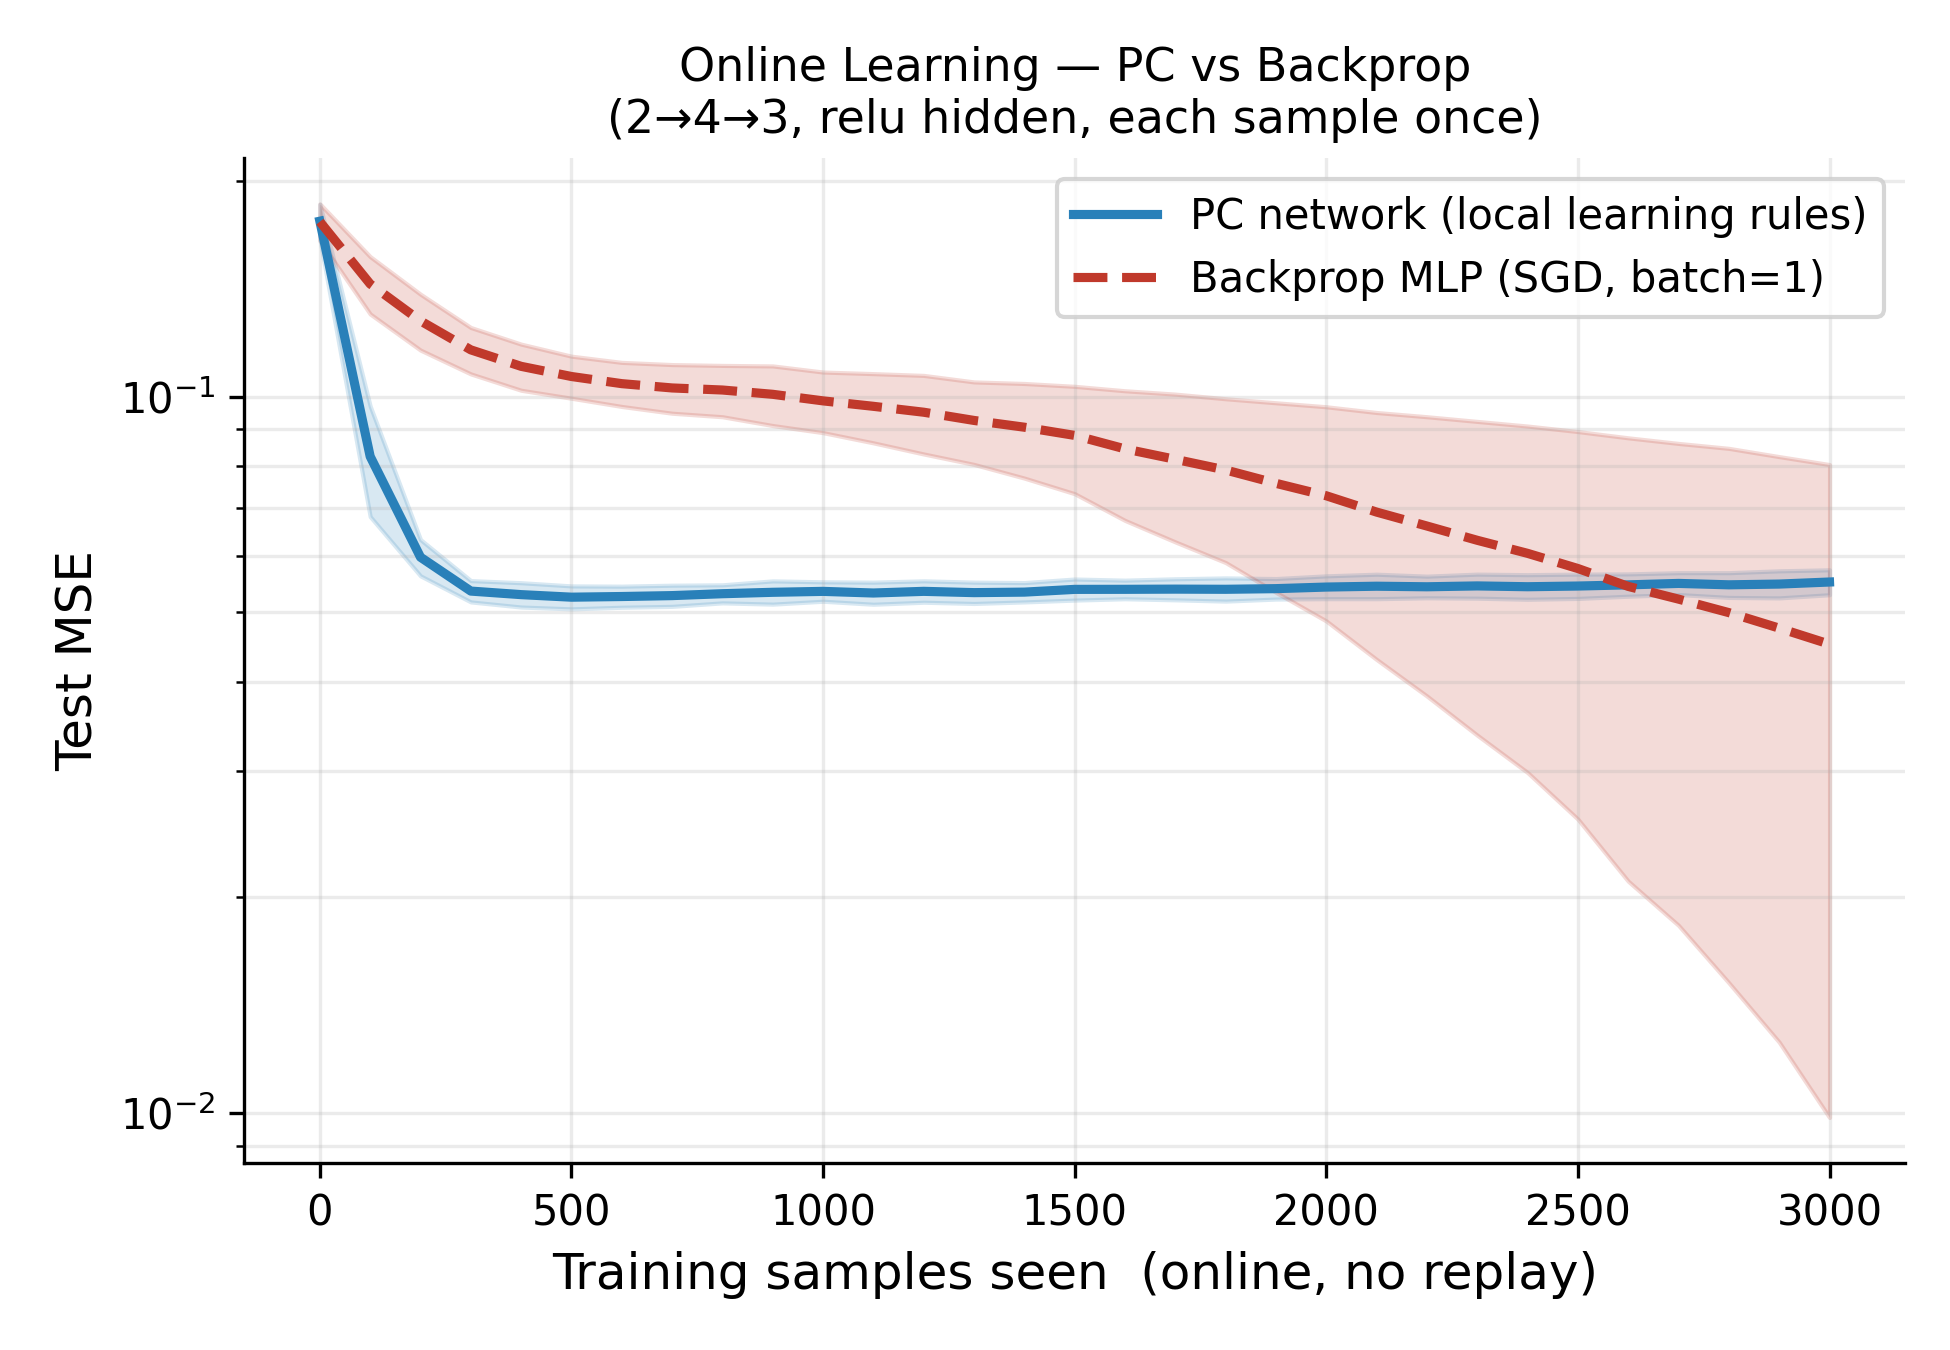
\includegraphics[width=0.75\linewidth]{figures/online_comparison_2x4x3_relu.png}
\caption{Online learning curves (no replay, one pass through data) for the
PC network and a matched backpropagation MLP.
Shaded bands show $\pm 1$ standard deviation across three seeds.
PC converges rapidly and consistently; backpropagation achieves a lower
mean final MSE but with considerably higher seed-to-seed variance.}
\label{fig:online_comparison}
\end{figure}

\subsection{Simulation fidelity validation}
\label{sec:exp-fidelity}

The RTL implementation operates in IEEE-754 float32, while the Python reference
uses float64. To bound this precision gap, a float32-emulating variant of the
Python reference is constructed by rounding all stored state (weights, biases,
neuron states, errors) to float32 after each tick, and rounding all inter-layer
inputs to float32 before each tick, while keeping intra-tick arithmetic in
float64. This emulation captures tick-boundary quantisation but not intra-tick
rounding, making it an \emph{upper bound} on the float64--RTL divergence: if
float64 and float32-emulated agree, the true RTL can only agree more closely.

Both variants run in parallel on the same \(2 \rightarrow 4 \rightarrow 3\)
network for 500 ticks (200 inference-only, 300 with weight updates), with the
per-tick divergence recorded in three metrics: state RMSE per layer, weight
matrix RMSE per layer, and worst-case maximum absolute difference across all
stored parameters (Figure~\ref{fig:fidelity_trace}).

The peak maximum absolute difference across all 500 ticks is
$4.77 \times 10^{-8}$, which is approximately the float32 unit of least
precision (ULP) for values near unity ($2^{-24} \approx 5.96 \times 10^{-8}$),
and it remains constant throughout both the inference and learning phases.
Weight matrix RMSE between the two variants stays in the range
$10^{-15}$--$10^{-12}$, confirming that accumulated tick-boundary rounding does
not compound over 500 steps. These results validate that the Python float64
reference faithfully predicts RTL float32 behaviour at the tick-level
granularity at which the correspondence is claimed.

\begin{figure}[H]
\centering
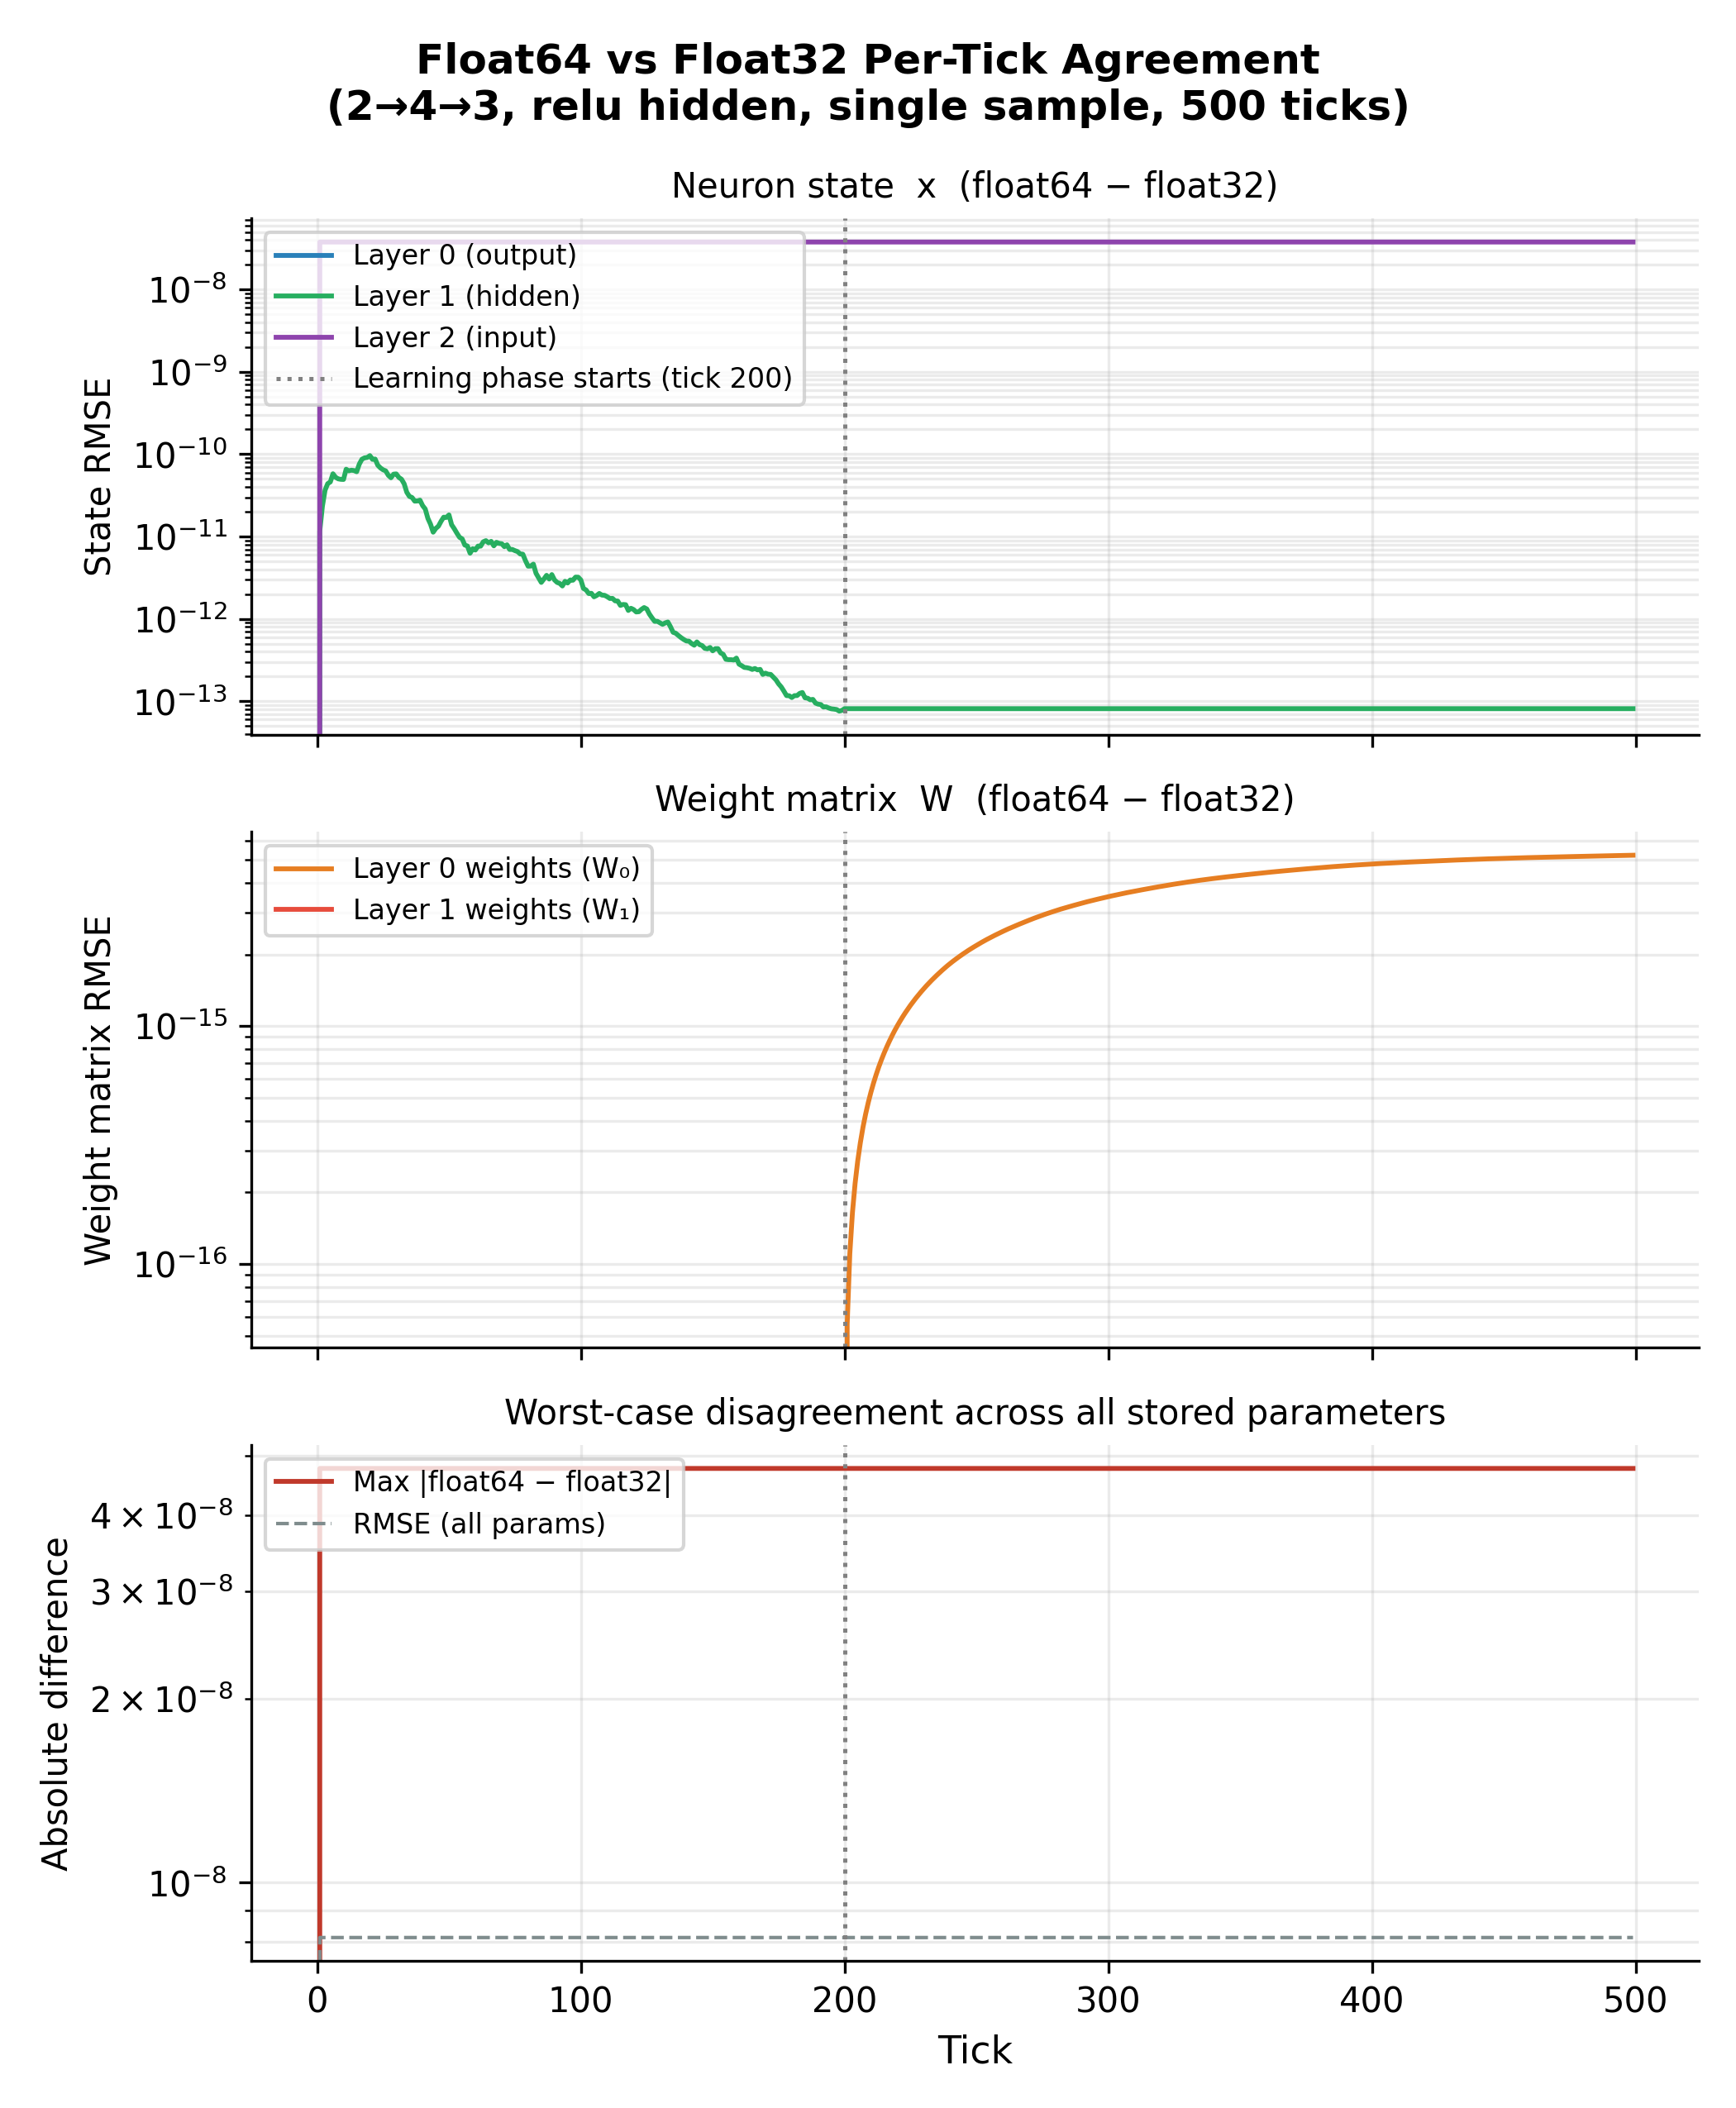
\includegraphics[width=0.82\linewidth]{figures/fidelity_trace_2x4x3_relu.png}
\caption{Per-tick agreement between float64 Python reference and float32-emulated
variant over 500 ticks (dashed vertical line marks the transition from inference
to learning phase at tick 200). Top: state RMSE per layer. Middle: weight matrix
RMSE per layer. Bottom: worst-case maximum absolute difference across all stored
parameters. The peak max difference of $4.77 \times 10^{-8}$ matches the float32
ULP floor and remains flat throughout both phases.}
\label{fig:fidelity_trace}
\end{figure}

\subsection{Quantitative summary}
\label{sec:exp-summary}

\begin{table}[H]
\centering
\begin{tabular}{lccc}
\hline
Experiment & Architecture & Initial MSE & Final MSE \\
\hline
Teacher--student (ReLU) & \(2 \rightarrow 4 \rightarrow 3\) & 0.341207 & 0.005935 \\
Hidden tanh             & \(2 \rightarrow 2 \rightarrow 1\) & 1.106512 & 0.004382 \\
\hline
Scaling: small  & \(2 \rightarrow 4 \rightarrow 3\)  & 0.1886 & 0.000380 \\
Scaling: medium & \(4 \rightarrow 8 \rightarrow 4\)  & 0.2179 & 0.000626 \\
Scaling: large  & \(8 \rightarrow 16 \rightarrow 8\) & 0.2819 & 0.000224 \\
\hline
Scaling (bias init): small  & \(2 \rightarrow 4 \rightarrow 3\)  & 0.4519 & 0.000501 \\
Scaling (bias init): medium & \(4 \rightarrow 8 \rightarrow 4\)  & 0.3804 & 0.000516 \\
Scaling (bias init): large  & \(8 \rightarrow 16 \rightarrow 8\) & 0.4771 & 0.000231 \\
\hline
\end{tabular}
\caption{Final MSE values reported at epoch~25. The top two rows are the
reference regression experiments (RTL simulation); the middle three are the
architectural scaling sweep (Python reference, sparse tiled tanh teacher,
zero bias init); the bottom three repeat the scaling sweep with bias weights
initialised from $\mathcal{N}(0,\,0.5^2)$.  Final residuals are comparable
across both bias-init conditions, confirming robustness of the local update
rule to non-zero bias offsets.}
\label{tab:results-summary}
\end{table}

Across all five runs, end-to-end supervised learning proceeds using only local
state variables, local prediction errors, and adjacent-layer communication
under a fixed FSM schedule. Nonzero residual floors in the RTL experiments
motivate further study of tick budget and step-size tuning.

\subsection{Evaluation protocol}

Learning proceeds in alternating phases: an \textbf{inference phase}
(\(\alpha = 0\), \(\gamma > 0\)) in which network state settles under clamped
boundary conditions, and a \textbf{learning phase} (\(\alpha > 0\),
\(\gamma > 0\)) in which weights are updated while state continues evolving.
The distinction is imposed entirely through boundary conditions and
learning-rate parameters, with no change to the internal hardware schedule.

\section{Discussion: Toward Embedded Adaptive Computation}
\label{sec:discussion}

The proposed system is motivated by a practical hardware question: what changes when learning is implemented as a local dynamical process rather than as a procedure that alternates between forward evaluation, backward gradient propagation, and parameter updates stored in centralized memory. Predictive coding is attractive in this context because its update rules decompose into strictly local terms, allowing each unit to update its state and synapses using only adjacent-layer signals. The resulting substrate resembles a distributed physical process more than a conventional program executed by a centralized controller.

This perspective shifts where task structure is expressed in the system. In a conventional von Neumann setting, task behavior is typically specified primarily through externally authored software executed on a fixed substrate. In the present architecture, behavior is shaped more directly by the interaction between inputs, local state dynamics, local plasticity, and externally imposed boundary conditions.

\subsection{Relationship to Mortal Computation}

Hinton introduces the concept of mortal computation to describe systems in which algorithm and hardware are inseparable: because each physical instance has unknown analog variations, the trained parameters are useful only for that particular piece of hardware and die with it \cite{hinton2022forward}. The present work sits closer to this end of the design space than to conventional immortal computation. The predictive-coding update rules are not software executing on a general-purpose substrate --- they are directly instantiated as the hardware datapath itself. The FSM schedule, the MAC accumulation, the local state registers, and the weight update logic are the process; there is no separation between hardware and software.
This framing is descriptive rather than foundational. The value is to highlight how a fixed local dynamical substrate can support both inference and adaptation without separate programmed learning phases --- a structural property it shares with the mortal-computation perspective, even though the present design uses synchronous digital logic rather than analog circuits. Whether extending this further toward true analog mortal computation --- accepting hardware-specific parameter fidelity in exchange for energy efficiency --- would benefit predictive-coding substrates is an open question for future work.

\subsection{Relationship to Moravec's Paradox}

Moravec's Paradox highlights an asymmetry between symbolic manipulation, which maps cleanly onto sequential digital computation, and sensorimotor inference, which is robust in biological systems but challenging for conventional architectures \cite{moravec1988mind}. The present work does not claim to resolve this paradox. Rather, it provides a concrete substrate for testing a related hypothesis: some aspects of perception and control may be better realized as fast local inference in distributed dynamical systems than as explicit symbolic computation mediated by global memory.

Because the proposed architecture performs continual local error minimization under fixed update rules, it may be well suited to tasks naturally expressed as inference under constraints, particularly in noisy, streaming, or partially observed settings. Substantiating this hypothesis requires empirical comparisons to conventional digital baselines under matched compute and energy budgets.

\subsection{Limitations and future directions}

Several limitations follow from the current design. First, the architecture reuses a sequential floating-point datapath that iterates over presynaptic indices, reducing area per neuron but increasing tick latency as fan-in grows. Second, synthesizable implementations of nonlinear activations and their derivatives require careful numerical design. Third, convergence and stability guarantees for the coupled discrete-time, finite-precision, clamped system are not implied by continuous-time analyses; stability regions should be mapped empirically and, where possible, analyzed theoretically.

Section~\ref{sec:exp-stability} provides this empirical characterization: a
grid sweep over 64 \((\alpha,\gamma)\) pairs finds that convergence is gated
primarily by a minimum inference step size \(\gamma \approx 0.07\), with no
divergence or oscillation observed across the tested range, and a tick-budget
sweep identifies diminishing-returns behavior with a practical knee near
\(T = 50\) inference ticks per sample.

These limitations motivate future work on architectural scaling (parallelism vs area/power), activation approximations suitable for synthesis, and task-driven benchmarks that identify regimes where local online inference is beneficial.

\appendix
\section{Reproducing the Experiments}

All experiments described in this paper can be reproduced using the public
repository.

\begin{verbatim}
git clone https://github.com/alskaf1293/neuralcomputer
cd neuralcomputer
./scripts/test_all.sh
\end{verbatim}

Running the script executes the full suite of simulation experiments.

Outputs are written as CSV files under the \texttt{runs/} directory. The
repository also provides Python scripts that generate the plots reported in
the paper from these outputs.

\section*{Acknowledgments}

I am especially grateful to Greg Ver Steeg for his encouragement and for many conversations that helped sustain this project from beginning to end.

\bibliographystyle{plain}
\bibliography{references}
\end{document}
